\documentclass[12pt, letterpaper]{article}

\usepackage{common/preamble}

\begin{document}

% common/portada.tex
\thispagestyle{empty} 

\begin{center}
	\vspace{0.8cm}
	
	% --- Logo Header ---
	\begin{minipage}{0.15\textwidth}
		\centering
		
\includegraphics[width=\textwidth]{UNAM} 
	\end{minipage}
	\hfill
	\begin{minipage}{0.65\textwidth}
		\centering
		{\color{black}\fontsize{16}{18}\selectfont
			\textbf{UNIVERSIDAD NACIONAL AUTÓNOMA DE MÉXICO} \\
			\vspace{0.3cm}
			\textbf{FACULTAD DE INGENIERÍA} \\
			\vspace{0.3cm}
			\textbf{PROYECTO FINAL DE BASES DE DATOS} \\
			\vspace{0.3cm}
			\textbf{SEMESTRE 2026 - 2}
		}
	\end{minipage}
	\hfill
	\begin{minipage}{0.15\textwidth}
		\centering
		
\includegraphics[width=\textwidth]{UNAM_INGENIERIA}
	\end{minipage}
	
	\vspace{1.2cm}
	
	% --- Institutional Divider ---
\begin{tikzpicture}
	\draw[unamgold, line width=1.5pt] (0,0) -- (0.3\textwidth,0);
	\draw[unamblue, line width=1.5pt] (0.3\textwidth,0) -- (0.99\textwidth,0);
\end{tikzpicture}
	
	\vspace{1.5cm}
	
	% --- Project Title ---
	{\color{black}\fontsize{20}{22}\selectfont
		\textbf{ECOBICI} \\
		\vspace{0.4cm}
		{\fontsize{16}{18}\selectfont \textbf{Sistema de Gestión de Movilidad Urbana}} \\
		\vspace{0.6cm}
		{\fontsize{14}{16}\selectfont \textbf{Documentación Técnica}}
	}
	
	\vspace{1.8cm}
	
	% --- Team Information ---
	{\color{black}\fontsize{12}{14}\selectfont
		\renewcommand{\arraystretch}{1.4} % Spacing for the table
		\begin{tabular}{r l}
			\textbf{Profesora:}   & M.I.A. Martha López Pelcastre \\
			\textbf{Equipo:}       & SQuipoL \\
			\textbf{Integrantes:}  & Díaz Antúnez David \\
			                      & Hernández Acosta Mauricio Gabriel \\
			                      & Sánchez Luján César Ricardo \\
		\end{tabular}
	}
	
	\vfill
	
	% --- Footer ---
	{\color{black}\fontsize{11}{13}\selectfont
		\textbf{Ciudad Universitaria, Ciudad de México} \hfill \textbf{31 de Mayo de 2026}
	}
\end{center}

\newpage

% Set numbering style and start counting
\pagenumbering{roman}

% --- Table of Contents ---
\tableofcontents
\newpage

% --- List of Figures ---
\listoffigures
\newpage

% Start page numbering in arabic for sections
\pagenumbering{arabic}

\section{Introducción}

La movilidad urbana representa uno de los principales desafíos en las grandes ciudades debido al crecimiento poblacional y al incremento constante de los medios de transporte. Como alternativa sustentable, los sistemas de bicicletas compartidas permiten a los usuarios desplazarse de manera eficiente, económica y amigable con el medio ambiente.

El presente proyecto consiste en el diseño e implementación de una base de datos para el sistema ECOBICI, cuyo objetivo es administrar la información relacionada con usuarios, membresías, estaciones, bicicletas, viajes, incidentes, métodos de pago y personal operativo. La base de datos fue desarrollada aplicando los principios del diseño conceptual, lógico y físico, garantizando la integridad, consistencia y disponibilidad de la información.

Asimismo, se implementaron mecanismos de seguridad, restricciones de integridad, procedimientos almacenados, funciones, vistas y disparadores que permiten automatizar procesos y asegurar el correcto funcionamiento del sistema. Finalmente, se desarrollaron consultas e informes estadísticos que facilitan la toma de decisiones dentro de la organización.

\section{Objetivos}

\subsection{Objetivo General}

Diseñar e implementar una base de datos relacional para el sistema ECOBICI que permita administrar de manera eficiente la información relacionada con usuarios, membresías, bicicletas, estaciones, viajes, incidentes y empleados, garantizando la integridad, seguridad y disponibilidad de los datos.

\subsection{Objetivos Específicos}

\begin{itemize}
	\item Diseñar el modelo entidad-relación del sistema ECOBICI.
	\item Construir el modelo relacional normalizado hasta Tercera Forma Normal.
	\item Implementar restricciones de integridad mediante llaves primarias, llaves foráneas, restricciones CHECK, UNIQUE y DEFAULT.
	\item Desarrollar procedimientos almacenados, funciones, vistas y disparadores para automatizar procesos.
	\item Implementar mecanismos de seguridad mediante usuarios y permisos.
	\item Generar consultas e informes estadísticos que apoyen la toma de decisiones.
\end{itemize}

\section{Descripción del Problema}

ECOBICI es un sistema de movilidad urbana basado en el préstamo y renta de bicicletas dentro de la Ciudad de México. El servicio permite a los usuarios adquirir diferentes tipos de membresías para acceder a las bicicletas disponibles en diversas estaciones distribuidas estratégicamente en la ciudad.

Debido al volumen de información generado por las operaciones diarias, resulta necesario contar con una base de datos capaz de administrar usuarios, membresías, métodos de pago, estaciones, bicicletas, viajes, incidentes y personal de la organización. Además, el sistema debe permitir mantener un historial de viajes, registrar accidentes e incidentes, controlar el inventario de bicicletas y estaciones, gestionar la información de los empleados y generar reportes estadísticos que apoyen la toma de decisiones.

Por lo anterior, se requiere diseñar e implementar una base de datos relacional que garantice la integridad, consistencia y disponibilidad de la información, permitiendo automatizar procesos operativos y administrativos mediante el uso de restricciones, procedimientos almacenados, funciones, vistas y disparadores.

\section{Reglas de Negocio}

\begin{enumerate}
	\item Cada usuario debe registrarse proporcionando nombre completo, fecha de nacimiento, correo electrónico, código de identificación oficial, género y al menos un teléfono de contacto.
	\item El correo electrónico de cada usuario debe ser único dentro del sistema.
	\item Todo usuario debe contar con una membresía activa para poder utilizar el servicio.
	\item Las membresías disponibles son Básica, Intermedia y Premium.
	\item Un usuario puede cambiar de membresía cuando lo desee.
	\item Todo usuario debe tener registrado al menos un método de pago activo mientras mantenga una suscripción vigente.
	\item La eliminación del último método de pago provoca la cancelación automática de la suscripción asociada.
	\item Para utilizar el servicio es obligatorio contar con una tarjeta de movilidad integrada asociada al usuario.
	\item Cada bicicleta posee un número de serie único que la identifica dentro del sistema.
	\item Las bicicletas pueden encontrarse en estado de funcionamiento, mantenimiento o baja.
	\item Cada bicicleta pertenece a una categoría de tamaño: chica, mediana o grande.
	\item Todo viaje debe registrar una estación de origen y una estación de destino.
	\item Cada viaje debe almacenar fecha, hora de inicio y hora de finalización.
	\item Todo viaje debe quedar almacenado en un historial permanente para fines estadísticos y administrativos.
	\item Los incidentes reportados deben asociarse a un viaje previamente registrado.
	\item Cada incidente debe registrar fecha, hora, ubicación y tipo de incidente.
	\item Las estaciones mantienen un inventario actualizado de bicicletas disponibles y terminales operativas.
	\item Todo empleado pertenece a un área específica de trabajo.
	\item Los empleados pueden pertenecer al área de mantenimiento o administración.
	\item Cada empleado debe contar con un RFC único.
	\item Las faltas de los empleados deben registrarse mediante un consecutivo individual por empleado.
	\item Cada falta debe registrar la fecha y el motivo correspondiente.
	\item El sistema debe conservar el historial de faltas de todos los empleados.
	\item Cada incidente atendido debe estar asociado a un agente responsable.
	\item El sistema debe generar información estadística relacionada con usuarios, bicicletas, estaciones, viajes, incidentes y empleados.
\end{enumerate}

\section{Modelo Entidad–Relación}

El Modelo Entidad–Relación representa la estructura conceptual de la base de datos desarrollada para el sistema ECOBICI. En este modelo se identifican las principales entidades involucradas en la operación del sistema, así como sus atributos y relaciones.

Las entidades modeladas permiten administrar la información relacionada con usuarios, membresías, bicicletas, estaciones, viajes, incidentes, métodos de pago y personal operativo. Asimismo, se establecen las cardinalidades necesarias para garantizar la correcta representación de las reglas de negocio identificadas durante la fase de análisis.

Como puede observarse en la Figura~\ref{fig:modelo_er}, el modelo conceptual permite identificar claramente las dependencias entre las entidades principales del sistema, sirviendo como base para la construcción del modelo relacional y la implementación física de la base de datos.

\begin{figure}[H]
	\centering
	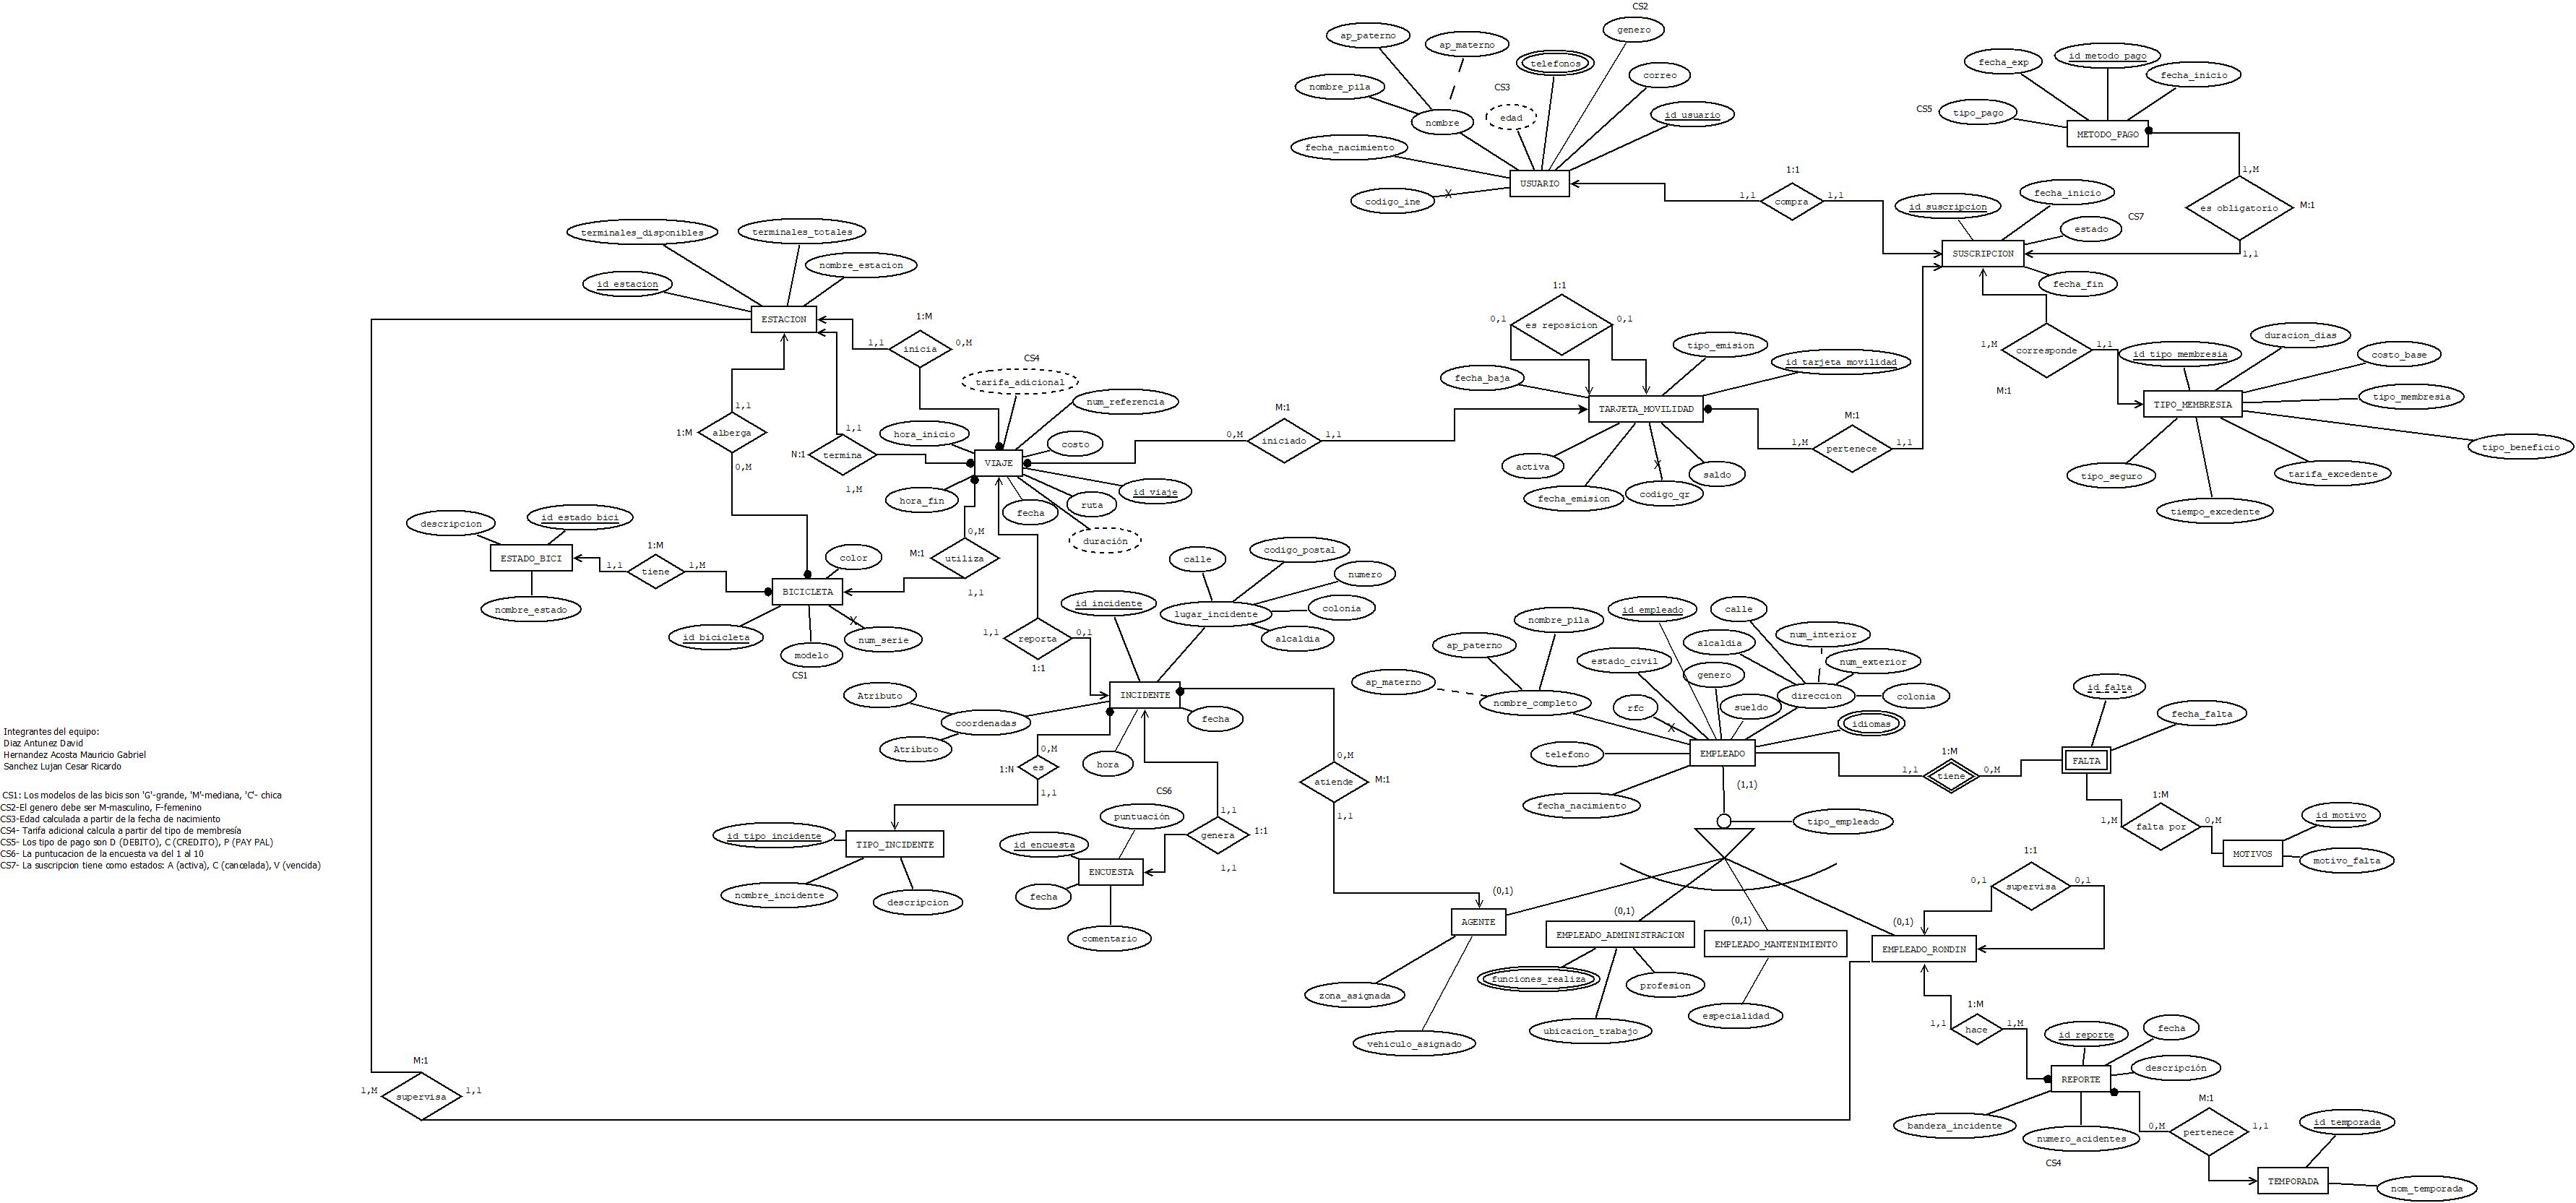
\includegraphics[width=0.9\textwidth]{figures/mer.jpg}
	\caption{Modelo Entidad–Relación del sistema ECOBICI}
	\label{fig:modelo_er}
\end{figure}

\section{Modelo Relacional}

El Modelo Relacional fue construido a partir del Modelo Entidad–Relación, transformando cada entidad en tablas y definiendo las relaciones mediante llaves primarias y llaves foráneas.

La estructura resultante se encuentra normalizada hasta la Tercera Forma Normal (3FN), reduciendo la redundancia de datos y garantizando la integridad referencial dentro del sistema.

Para facilitar la organización de la información, la base de datos fue dividida en distintos esquemas que agrupan tablas con funciones similares, tales como \texttt{catalogo}, \texttt{usuarios}, \texttt{movilidad}, \texttt{personal}, \texttt{incidentes} y \texttt{reportes}.

La Figura~\ref{fig:modelo_relacional} muestra la estructura lógica completa de la base de datos, incluyendo las tablas, atributos, llaves primarias, llaves foráneas y relaciones existentes entre los diferentes componentes del sistema.

\begin{figure}[H]
	\centering
	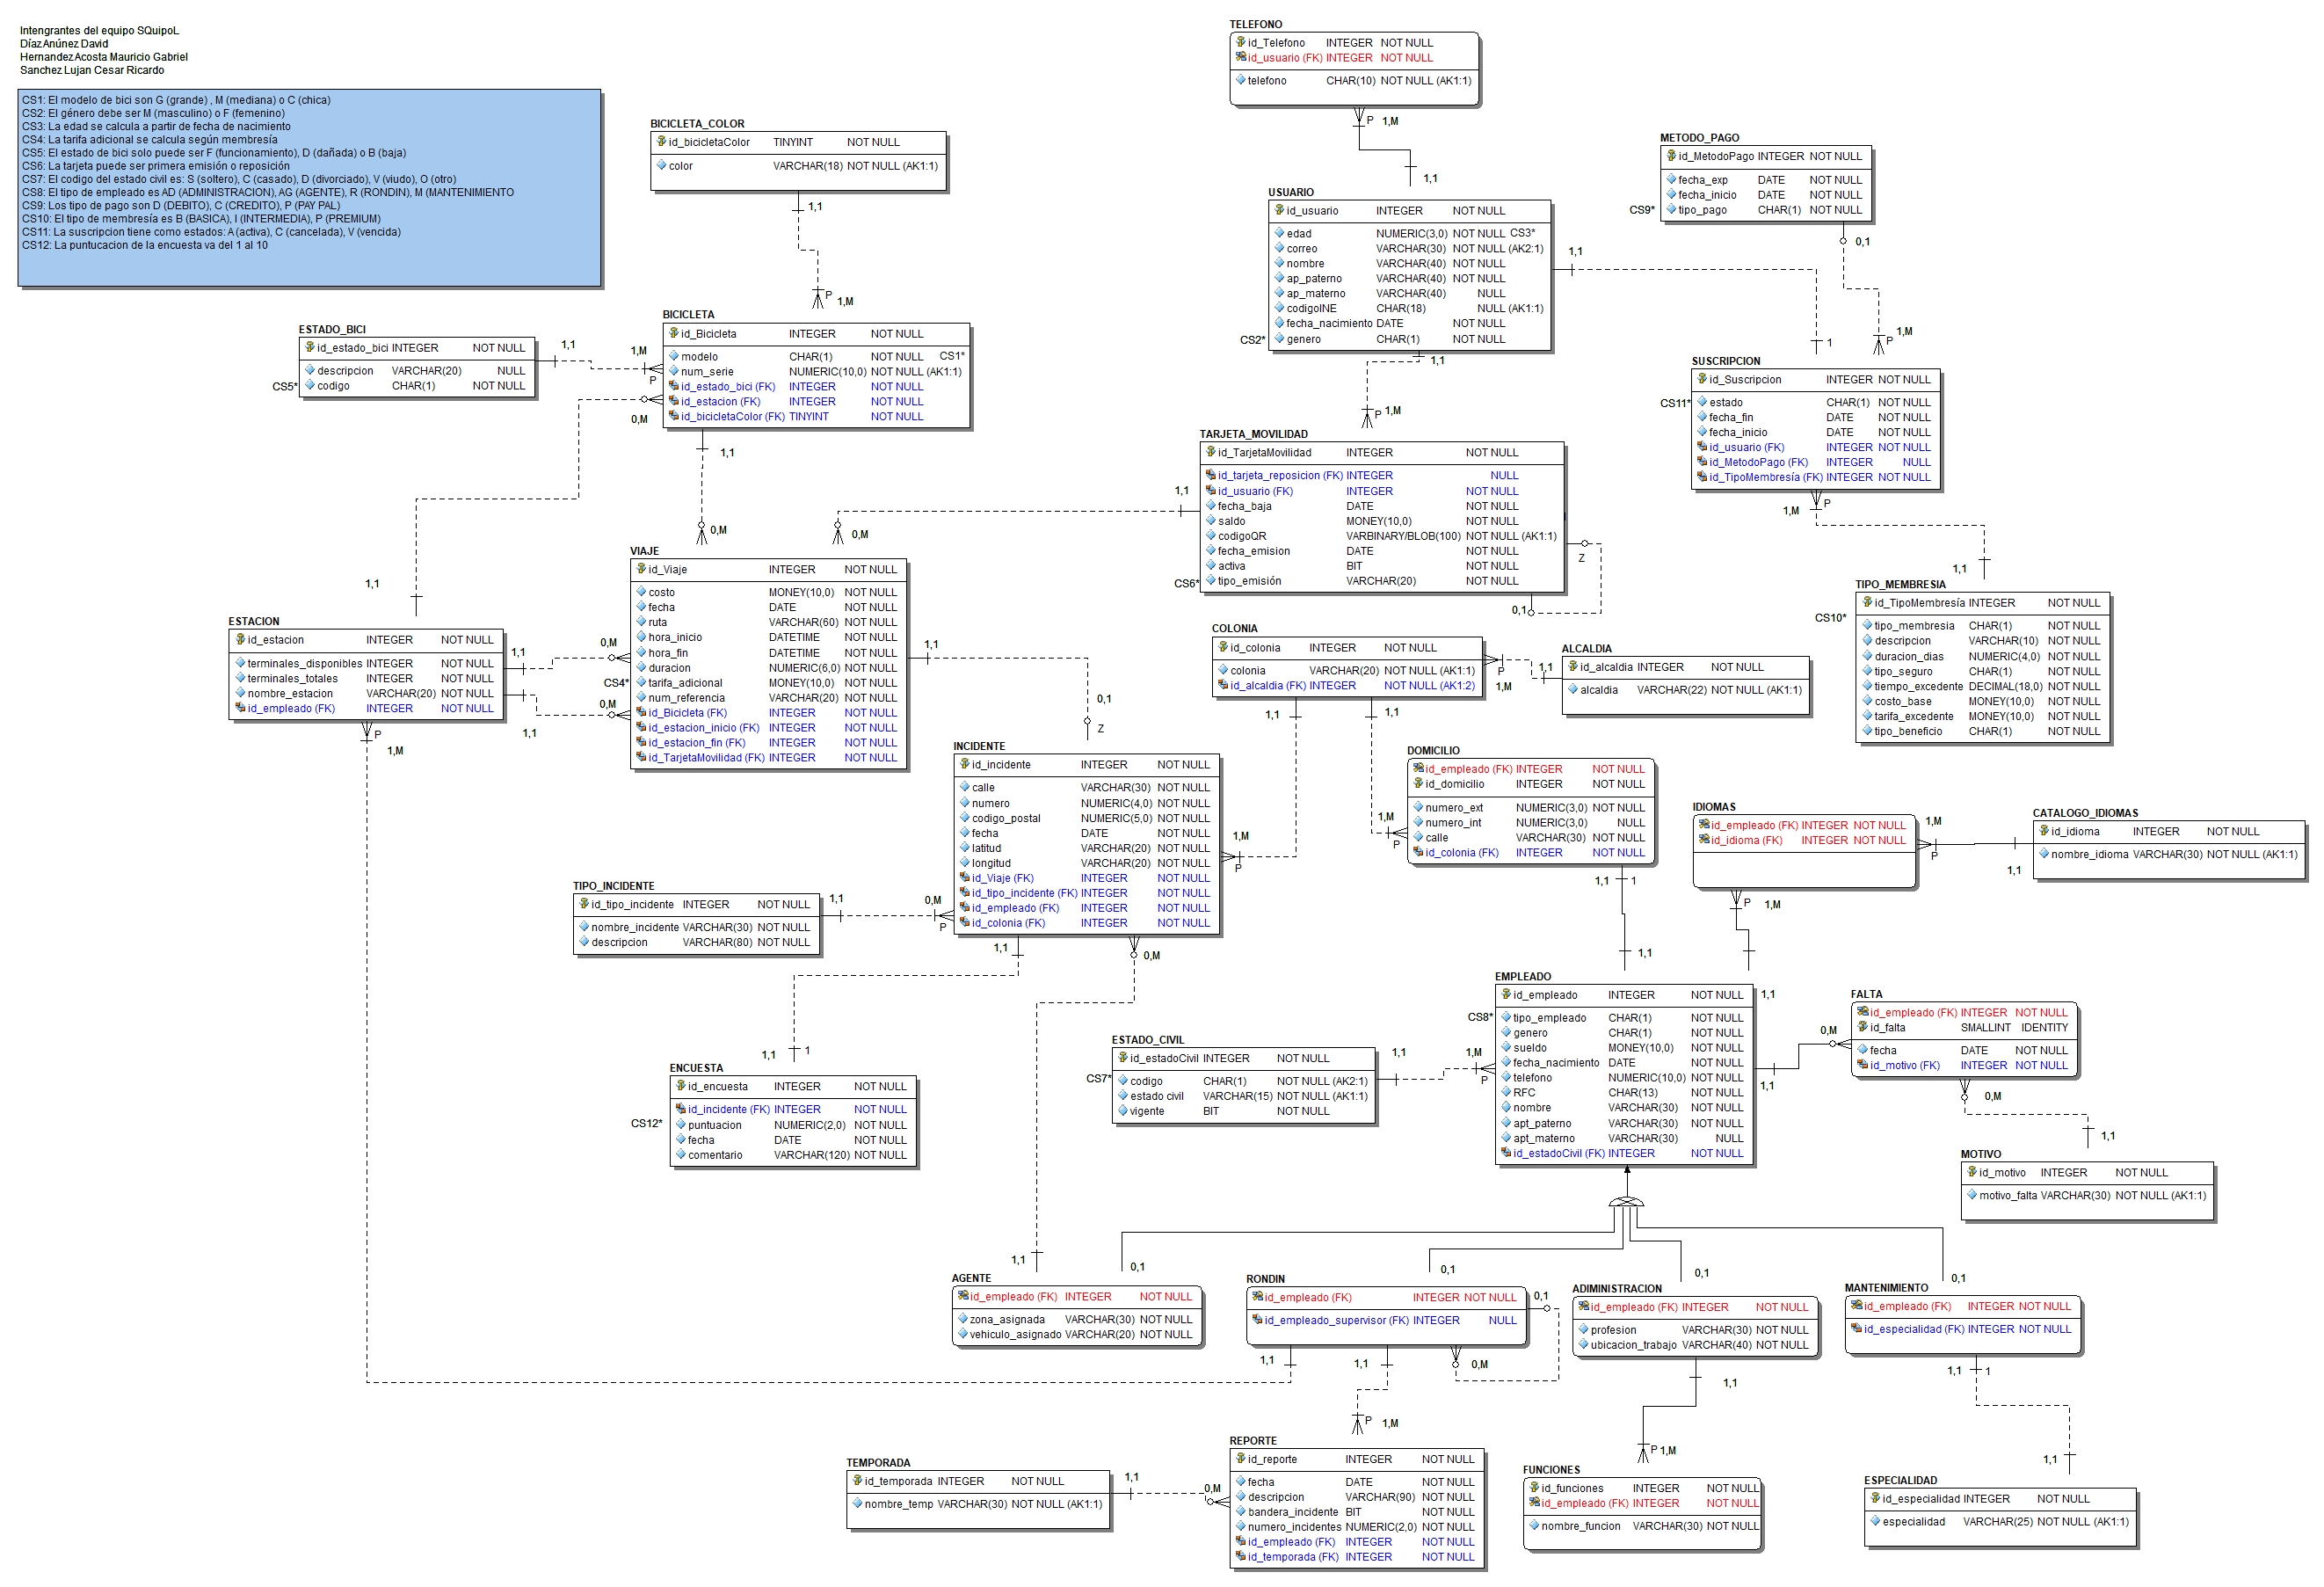
\includegraphics[width=0.9\textwidth]{figures/mr.jpg}
	\caption{Modelo Relacional del sistema ECOBICI}
	\label{fig:modelo_relacional}
\end{figure}

\section{Normalización}

Durante la etapa de diseño de la base de datos se aplicaron desde el inicio los principios de normalización vistos en el curso, por lo que el modelo fue construido directamente considerando las reglas necesarias para cumplir con la Tercera Forma Normal (3FN). Debido a este enfoque, no fue necesario realizar un proceso posterior de descomposición de tablas, ya que las entidades y relaciones fueron definidas desde el principio evitando redundancias y dependencias innecesarias.

\subsection{Primera Forma Normal (1FN)}

La Primera Forma Normal establece que todos los atributos deben contener valores atómicos y que no deben existir grupos repetitivos dentro de una misma tabla. Durante el diseño de la base de datos se procuró que cada atributo almacenara únicamente un valor indivisible y que cada registro pudiera identificarse de manera única mediante una clave primaria.

Por ejemplo, la información correspondiente a teléfonos de usuarios se almacenó en una tabla independiente, permitiendo registrar múltiples números telefónicos para un mismo usuario sin generar grupos repetitivos dentro de la tabla principal de usuarios.

De esta manera, todas las tablas cumplen con los requisitos establecidos por la Primera Forma Normal.

\subsection{Segunda Forma Normal (2FN)}

La Segunda Forma Normal establece que todos los atributos no clave deben depender completamente de la clave primaria de la tabla. Durante el diseño se identificaron adecuadamente las entidades principales y se separó la información en tablas especializadas para evitar dependencias parciales.

Cada tabla fue diseñada para representar una única entidad o concepto del sistema, garantizando que todos sus atributos describieran exclusivamente a la clave primaria correspondiente. Esto permitió evitar redundancias y mantener una estructura consistente para el almacenamiento de la información.

Por lo anterior, el modelo cumple con los requisitos de la Segunda Forma Normal.

\subsection{Tercera Forma Normal (3FN)}

La Tercera Forma Normal establece que no deben existir dependencias transitivas entre atributos que no forman parte de la clave primaria. Para cumplir este criterio, la información descriptiva y los valores reutilizables fueron separados en entidades independientes.

Durante las etapas finales del proyecto se incorporaron diversos catálogos para representar información de referencia utilizada por múltiples tablas. Entre ellos se encuentran los catálogos de alcaldías, estados civiles, idiomas, especialidades, motivos de faltas, estados de bicicletas, colores de bicicletas y tipos de incidentes.

La utilización de estos catálogos permitió centralizar la información, reducir la redundancia de datos y fortalecer la integridad referencial mediante el uso de llaves foráneas. Como resultado, la base de datos mantiene una estructura organizada, flexible y consistente.

Por las características descritas anteriormente, se concluye que el modelo relacional desarrollado para ECOBICI cumple con los principios de la Tercera Forma Normal (3FN), garantizando una adecuada organización de los datos y minimizando problemas de actualización, inserción y eliminación.

\section{Diccionario de Datos}

Debido a la cantidad de entidades y atributos presentes en el sistema ECOBICI, el diccionario de datos completo se presenta en el Anexo A. Dicho documento contiene la descripción detallada de las tablas, campos y tipos de datos que conforman la base de datos.

\section{Diseño Físico de la Base de Datos}

La implementación física de la base de datos ECOBICI se realizó utilizando SQL Server. Durante esta etapa se definieron los esquemas, tablas, restricciones, usuarios, permisos y objetos programados necesarios para garantizar el correcto funcionamiento del sistema.

El diseño físico fue desarrollado tomando como base el modelo relacional previamente definido, incorporando mecanismos que permiten asegurar la integridad de los datos, optimizar el acceso a la información y automatizar diversos procesos operativos.

\subsection{Seguridad}

La seguridad de la base de datos fue implementada mediante la creación de usuarios con distintos niveles de acceso, permitiendo controlar las operaciones que cada tipo de usuario puede realizar sobre la información almacenada.

Se definieron perfiles orientados a consulta, gestión y administración, con el objetivo de aplicar el principio de privilegios mínimos y garantizar la protección de los datos del sistema.

La creación de usuarios, asignación de permisos y configuración de seguridad se encuentran implementadas en el archivo \texttt{seguridad.sql}.

\subsection{Creación de la Base de Datos}

La estructura principal de la base de datos fue implementada en el archivo \texttt{creaBase.sql}. En este script se definieron los esquemas, tablas, llaves primarias, llaves foráneas y restricciones necesarias para garantizar la integridad de la información.

Para facilitar la organización de los datos, las tablas fueron agrupadas en distintos esquemas de acuerdo con su función dentro del sistema:
\begin{itemize}
	\item \textbf{catalogo:} Catálogos utilizados por múltiples módulos del sistema.
	\item \textbf{usuarios:} Información de usuarios y teléfonos de contacto.
	\item \textbf{movilidad:} Gestión de membresías, bicicletas, estaciones y viajes.
	\item \textbf{personal:} Información de empleados y recursos humanos.
	\item \textbf{incidentes:} Registro de incidentes y encuestas de satisfacción.
	\item \textbf{reportes:} Información relacionada con temporadas y reportes operativos.
\end{itemize}

Asimismo, se implementaron restricciones de integridad referencial mediante llaves foráneas, restricciones de dominio mediante cláusulas CHECK, validaciones de unicidad mediante restricciones UNIQUE y valores predeterminados mediante restricciones DEFAULT.

\subsection{Objetos Programados}

Con el propósito de automatizar procesos y facilitar la explotación de la información, se desarrollaron diversos objetos programados dentro de la base de datos.

Entre los objetos implementados se encuentran:
\begin{itemize}
	\item Procedimientos almacenados para operaciones de inserción, actualización y consulta (operaciones ABC, reposición de tarjetas, recargas, etc.).
	\item Funciones (UDFs) para realizar cálculos y obtener información derivada (edad, meses de membresía, tarifas excedentes).
	\item Vistas para simplificar consultas frecuentes (tarifa adicional de viajes, planes activos, resumen de incidentes).
	\item Triggers para automatizar validaciones y acciones relacionadas con modificaciones de datos.
\end{itemize}

La implementación de estos componentes se encuentra contenida en el archivo \texttt{dml.sql}, permitiendo centralizar la lógica de negocio dentro de la base de datos y mejorar la consistencia de las operaciones realizadas por el sistema.

\section{Carga Inicial}

Con el objetivo de validar el correcto funcionamiento de la base de datos y de los diferentes procesos implementados, se realizó una carga inicial de información representativa del sistema ECOBICI. Los datos cargados permiten probar la integridad de las relaciones, las restricciones definidas y las consultas estadísticas requeridas para el proyecto.

La carga inicial fue implementada mediante el archivo \texttt{cargaInicial.sql}, el cual contiene los registros necesarios para poblar las tablas principales de la base de datos.

Entre los datos cargados se encuentran:
\begin{itemize}
	\item Catálogos generales utilizados por los distintos módulos del sistema, tales como alcaldías, estados civiles, idiomas, especialidades, estados de bicicletas, colores de bicicletas, tipos de incidentes y motivos de faltas.
	\item Usuarios registrados dentro de la plataforma junto con su información personal y medios de contacto.
	\item Métodos de pago, membresías, suscripciones y tarjetas de movilidad asociadas a los usuarios.
	\item Estaciones ECOBICI distribuidas en diferentes ubicaciones de la ciudad.
	\item Bicicletas registradas dentro del inventario general del sistema, incluyendo su estado operativo, color y tamaño.
	\item Viajes realizados por los usuarios entre distintas estaciones, permitiendo generar históricos de recorridos y estadísticas de uso.
	\item Empleados pertenecientes a las diferentes áreas operativas y administrativas de la organización.
	\item Agentes encargados de la atención de incidentes y personal responsable de realizar rondines.
	\item Incidentes reportados por los usuarios durante los viajes y las encuestas asociadas a la atención brindada.
	\item Reportes operativos generados por el personal encargado de los rondines.
\end{itemize}

La información cargada fue diseñada para cubrir los distintos escenarios contemplados en los requerimientos del proyecto, permitiendo ejecutar correctamente los procedimientos almacenados, funciones, vistas, triggers e informes estadísticos desarrollados para la base de datos.

Asimismo, la carga inicial facilita la validación de las relaciones entre tablas y el comportamiento de las restricciones de integridad implementadas durante el diseño físico del sistema.

\section{Aplicación de Consideraciones}

Durante el desarrollo de la base de datos ECOBICI se aplicaron las consideraciones técnicas solicitadas en los requerimientos del proyecto. Estas consideraciones permitieron garantizar la integridad, consistencia, seguridad y rendimiento de la información almacenada.

\subsection{Lineamientos de Nomenclatura}

Con el propósito de mantener uniformidad en el desarrollo de la base de datos, se utilizaron convenciones de nomenclatura para los diferentes objetos implementados:
\begin{itemize}
	\item \texttt{pk\_}: Llaves primarias.
	\item \texttt{fk\_}: Llaves foráneas.
	\item \texttt{ck\_}: Restricciones CHECK.
	\item \texttt{u\_}: Restricciones UNIQUE.
	\item \texttt{idx\_}: Índices.
	\item \texttt{trg\_}: Disparadores (Triggers).
	\item \texttt{sp\_}: Procedimientos almacenados.
	\item \texttt{fn\_}: Funciones.
	\item \texttt{vw\_}: Vistas.
\end{itemize}

\subsection{Restricciones CHECK}

Se implementaron restricciones CHECK para validar los valores permitidos en distintos atributos del sistema, asegurando la integridad del dominio:
\begin{itemize}
	\item Validación de códigos para los estados de las bicicletas (e.g. \texttt{F}, \texttt{D}, \texttt{B}).
	\item Validación de los tipos de empleado permitidos (e.g. \texttt{a}, \texttt{r}, \texttt{d}, \texttt{m}).
	\item Validación del género de los empleados y usuarios (\texttt{M} o \texttt{F}).
	\item Validación de sueldos mayores a cero.
	\item Validación de puntuación de encuestas (rango de 1 a 10).
\end{itemize}

\subsection{Restricciones UNIQUE}

Se utilizaron restricciones UNIQUE para evitar la duplicidad de información crítica no clave primaria dentro de las tablas:
\begin{itemize}
	\item RFC y teléfono de los empleados.
	\item Correo electrónico e INE de los usuarios.
	\item Código de estado de bicicleta y de estado civil.
	\item Número de serie de la bicicleta.
\end{itemize}

\subsection{Restricciones DEFAULT}

Se implementaron valores predeterminados para simplificar el registro de información y garantizar la consistencia de ciertos atributos cuando no se proporciona un valor explícito:
\begin{itemize}
	\item Saldo inicial de la tarjeta de movilidad igual a 0 (\texttt{saldo DECIMAL(10,2) NOT NULL DEFAULT 0}).
	\item Fecha de emisión de tarjeta de movilidad igual a la fecha del sistema (\texttt{DEFAULT GETDATE()}).
	\item Fecha de encuesta de satisfacción igual a la fecha del sistema.
	\item Banderas y contadores de incidentes en reportes con valor predeterminado de 0.
\end{itemize}

\subsection{Llaves Artificiales}

La mayoría de las entidades utilizan identificadores numéricos (\texttt{id\_*}) como llaves primarias, facilitando la administración de relaciones y mejorando el rendimiento de las consultas y las operaciones de unión (JOIN).

\subsection{Llaves Naturales}

Se utilizaron llaves naturales complementarias cuando los atributos poseían significado y valor de identificación propio y único dentro del negocio:
\begin{itemize}
	\item RFC para los empleados.
	\item Código INE para los usuarios.
	\item Número de serie para las bicicletas.
\end{itemize}

\subsection{Columna Calculada}

Se implementó una columna calculada dentro de las tablas principales para simplificar el cálculo en consultas en tiempo real:
\begin{itemize}
	\item Campo \texttt{edad} en la tabla \texttt{personal.empleado} y \texttt{usuarios.usuario} calculada a partir de su fecha de nacimiento: \texttt{edad AS DATEDIFF(YEAR, fecha\_nacimiento, GETDATE())}.
	\item Campo \texttt{duracion} en la tabla \texttt{movilidad.viaje} calculada en minutos como la diferencia entre la hora de inicio y fin: \texttt{duracion AS DATEDIFF(MINUTE, hora\_inicio, hora\_fin)}.
\end{itemize}

\subsection{Índices}

Se implementaron índices no agrupados (\textit{Non-Clustered Indexes}) para optimizar el desempeño de las consultas más frecuentes realizadas sobre la base de datos:
\begin{itemize}
	\item \texttt{idx\_viaje\_fecha} sobre \texttt{movilidad.viaje(fecha)}.
	\item \texttt{idx\_incidente\_fecha} sobre \texttt{incidentes.incidente(fecha)}.
	\item \texttt{idx\_suscripcion\_usuario} sobre \texttt{movilidad.suscripcion(id\_usuario)}.
	\item \texttt{idx\_usuario\_nombre} sobre \texttt{usuarios.usuario(nombre, ap\_paterno)}.
	\item \texttt{idx\_empleado\_rfc} sobre \texttt{personal.empleado(RFC)}.
\end{itemize}

\subsection{Integridad Referencial}

La integridad referencial se garantizó mediante la adecuada declaración de llaves foráneas en todo el modelo relacional, asegurando que no existan registros huérfanos y que las relaciones correspondan estrictamente a lo establecido en las reglas de negocio.

\subsection{Borrado en Cascada}

Se implementó la cláusula \texttt{ON DELETE CASCADE} en las relaciones de las tablas secundarias que dependen directamente de una entidad principal. Esto permite eliminar automáticamente los registros relacionados cuando una entidad principal es eliminada del sistema, evitando la existencia de registros huérfanos. Las tablas dependientes del borrado de empleados y usuarios son:
\begin{itemize}
	\item \texttt{personal.administracion}
	\item \texttt{personal.agente}
	\item \texttt{personal.rondin}
	\item \texttt{personal.mantenimiento}
	\item \texttt{personal.domicilio}
	\item \texttt{personal.idiomas}
	\item \texttt{personal.falta}
	\item \texttt{usuarios.telefono}
	\item \texttt{movilidad.suscripcion}
	\item \texttt{movilidad.tarjeta\_movilidad}
	\item \texttt{movilidad.viaje}
\end{itemize}

\subsection{Procedimientos Almacenados}

Se desarrollaron procedimientos almacenados transaccionales (con bloqueos \texttt{TRY...CATCH} y transacciones \texttt{BEGIN TRAN / COMMIT / ROLLBACK}) para realizar operaciones de inserción, actualización, eliminación y generación de información estadística requerida por el sistema de manera consistente.

\subsection{Funciones}

Se implementaron funciones para encapsular lógica reutilizable y facilitar cálculos utilizados por distintos componentes de la base de datos, como la edad (\texttt{fn\_calcular\_edad}), meses de membresía (\texttt{fn\_meses\_membresia}) o tarifa excedente de viajes (\texttt{fn\_calcular\_tarifa\_excedente}).

\subsection{Vistas}

Se desarrollaron vistas para simplificar consultas complejas y facilitar el acceso a información consolidada:
\begin{itemize}
	\item \texttt{movilidad.vw\_viaje\_tarifa\_adicional}: Resuelve el cálculo de cargos excedentes por viaje en base a la membresía.
	\item \texttt{usuarios.vw\_usuarios\_planes\_activos}: Consolida la información de usuarios que poseen suscripciones activas.
	\item \texttt{incidentes.vw\_resumen\_incidentes}: Genera el listado y detalle de los reportes viales y mecánicos atendidos.
\end{itemize}

\subsection{Triggers}

Se implementaron triggers para automatizar procesos de validación y actualización de información ante eventos de inserción, modificación o eliminación de datos:
\begin{itemize}
	\item \texttt{trg\_viaje\_actualiza\_ubicacion\_bicicleta}: Actualiza la estación final en la tabla de bicicletas cuando finaliza un viaje.
	\item \texttt{trg\_metodo\_pago\_cancela\_suscripcion}: Cancela la suscripción activa si se elimina su método de pago único.
	\item \texttt{trg\_incidente\_marca\_bicicleta}: Marca automáticamente una bicicleta como dañada si se reporta un incidente mecánico grave.
	\item \texttt{trg\_viaje\_valida\_bicicleta\_operativa}: Evita el préstamo de bicicletas en estado de mantenimiento o dadas de baja.
	\item \texttt{trg\_tarjeta\_desactiva\_por\_reposicion}: Desactiva y da de baja la tarjeta anterior al emitir una reposición.
\end{itemize}

\subsection{Consultas Avanzadas}

Los informes estadísticos utilizan diferentes técnicas de consulta avanzadas:
\begin{itemize}
	\item Cláusulas de unión \texttt{INNER JOIN} y \texttt{LEFT JOIN}.
	\item Funciones de agregación como \texttt{COUNT}, \texttt{SUM} y \texttt{AVG}.
	\item Estructuras condicionales \texttt{CASE} y subconsultas complejas.
	\item Agrupamiento mediante \texttt{GROUP BY} y filtros post-agregación mediante \texttt{HAVING}.
\end{itemize}

\section{Informes y Estadísticas}

En esta sección se describen los quince informes y estadísticas requeridos para la administración y operación del sistema ECOBICI. Para cada informe se detalla el objetivo de la consulta, seguido del resultado obtenido en la ejecución del script correspondiente.

\subsection{Estadística 1. Daños en bicicletas con mayor frecuencia}

Esta consulta identifica las bicicletas que han estado involucradas en un mayor número de incidentes registrados. La información obtenida permite detectar unidades con problemas recurrentes y apoyar la toma de decisiones relacionadas con mantenimiento preventivo o sustitución de bicicletas.

\begin{figure}[H]
	\centering
	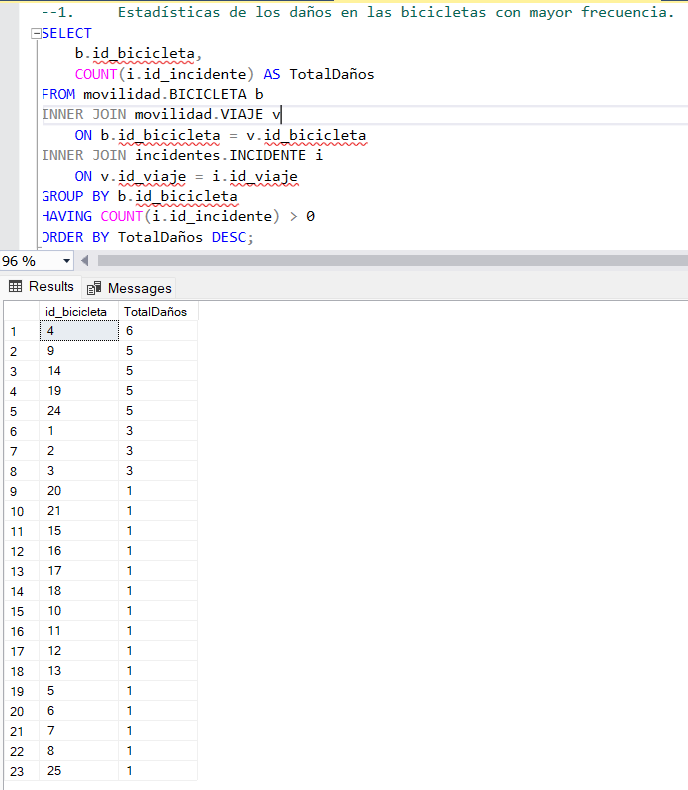
\includegraphics[width=0.85\textwidth]{figures/fig-004.png}
	\caption{Daños en bicicletas con mayor frecuencia}
	\label{fig:est_1}
\end{figure}

\subsection{Estadística 2. Top 5 de accidentes más frecuentes}

Esta consulta muestra los cinco tipos de incidentes que ocurren con mayor frecuencia dentro del sistema ECOBICI. Los resultados permiten identificar los riesgos más comunes y diseñar estrategias de prevención.

\begin{figure}[H]
	\centering
	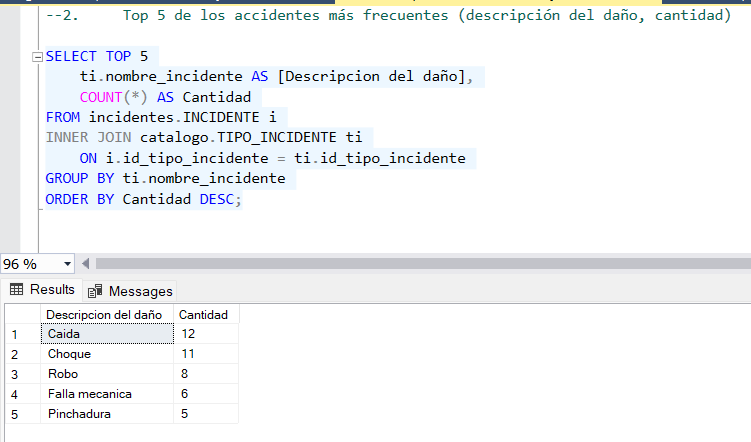
\includegraphics[width=0.85\textwidth]{figures/fig-005.png}
	\caption{Top 5 de accidentes más frecuentes}
	\label{fig:est_2}
\end{figure}

\subsection{Estadística 3. Estaciones con más reportes de accidentes}

Esta consulta presenta las estaciones que registran la mayor cantidad de accidentes durante un periodo determinado, agrupando la información por año y mes. Los resultados ayudan a identificar zonas de mayor riesgo operativo.

\begin{figure}[H]
	\centering
	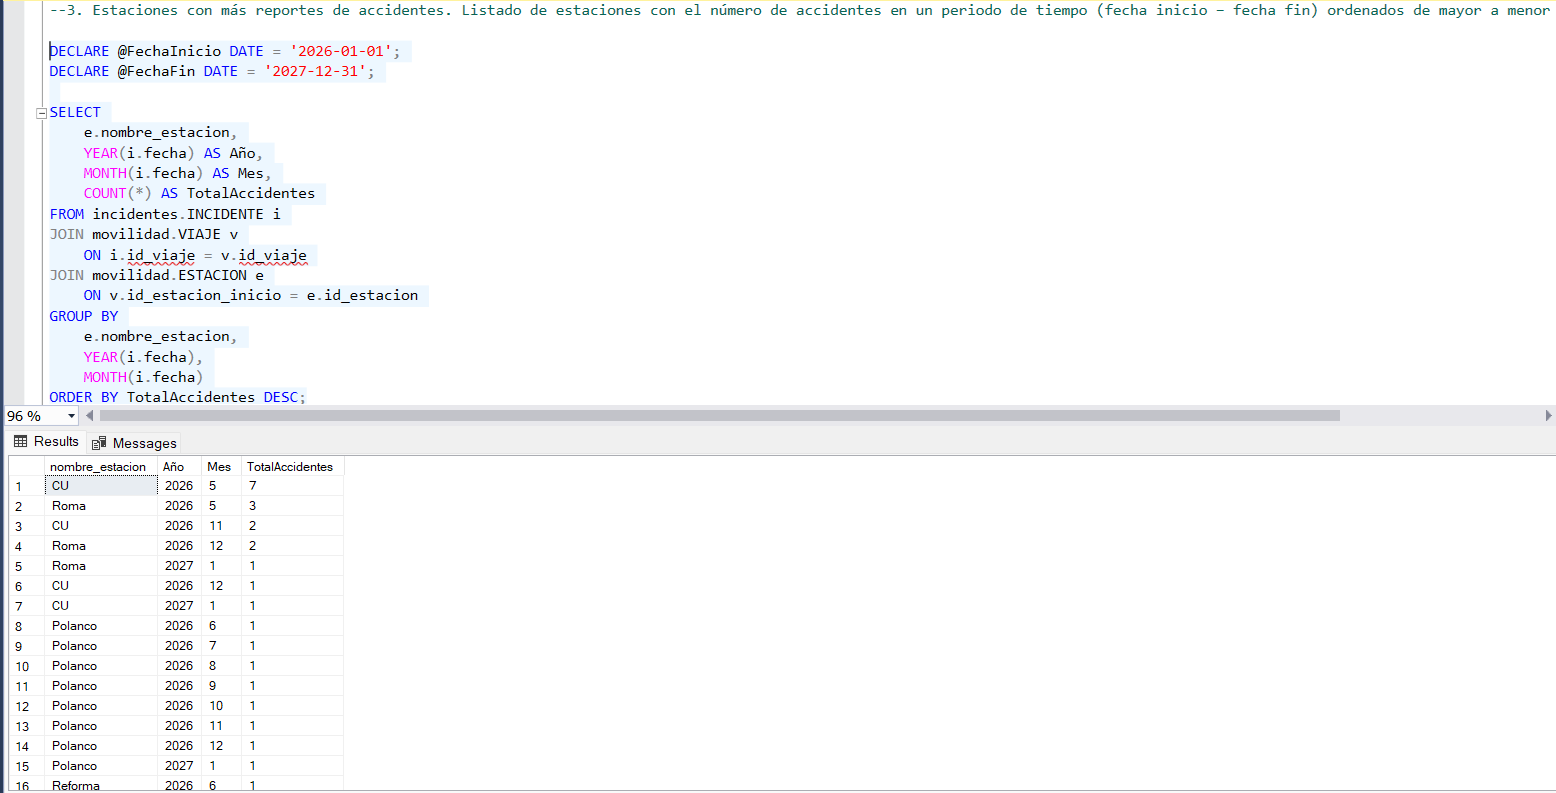
\includegraphics[width=0.85\textwidth]{figures/fig-006.png}
	\caption{Estaciones con más reportes de accidentes}
	\label{fig:est_3}
\end{figure}

\subsection{Estadística 4. Total de accidentes por mes y tipo}

Esta consulta muestra el número de accidentes registrados por mes y tipo de incidente. La información permite analizar tendencias temporales y evaluar el comportamiento de los diferentes tipos de accidentes.

\begin{figure}[H]
	\centering
	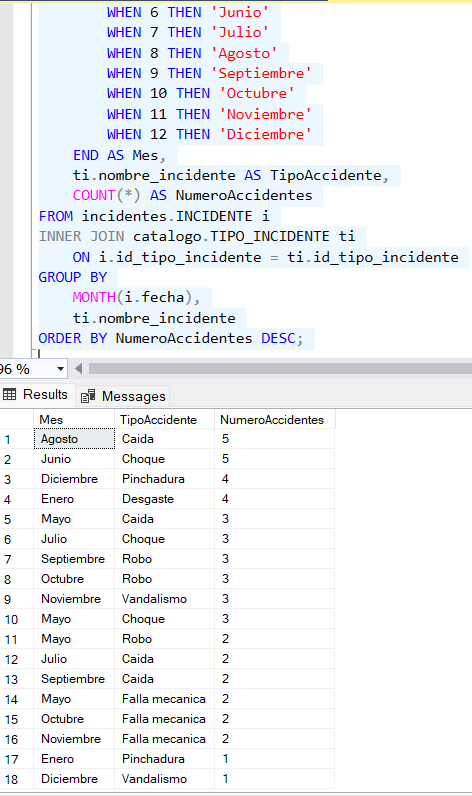
\includegraphics[width=0.85\textwidth]{figures/fig-007.png}
	\caption{Total de accidentes por mes y tipo}
	\label{fig:est_4}
\end{figure}

\subsection{Estadística 5. Usuarios por rango de edad}

Esta consulta clasifica a los usuarios por rangos de edad y tipo de membresía. Su objetivo es conocer la distribución demográfica de los usuarios del sistema.

\begin{figure}[H]
	\centering
	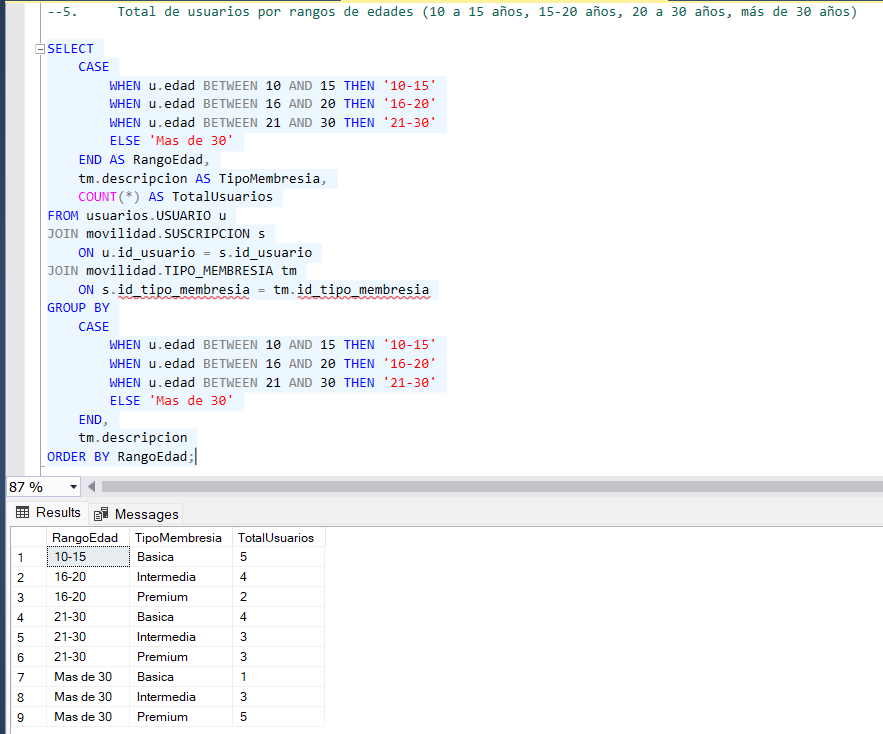
\includegraphics[width=0.85\textwidth]{figures/fig-008.png}
	\caption{Usuarios por rango de edad}
	\label{fig:est_5}
\end{figure}

\subsection{Estadística 6. Inventario de bicicletas por estación}

Esta consulta muestra el inventario de bicicletas por estación, incluyendo estado, color, cantidad de viajes realizados y número de accidentes asociados.

\begin{figure}[H]
	\centering
	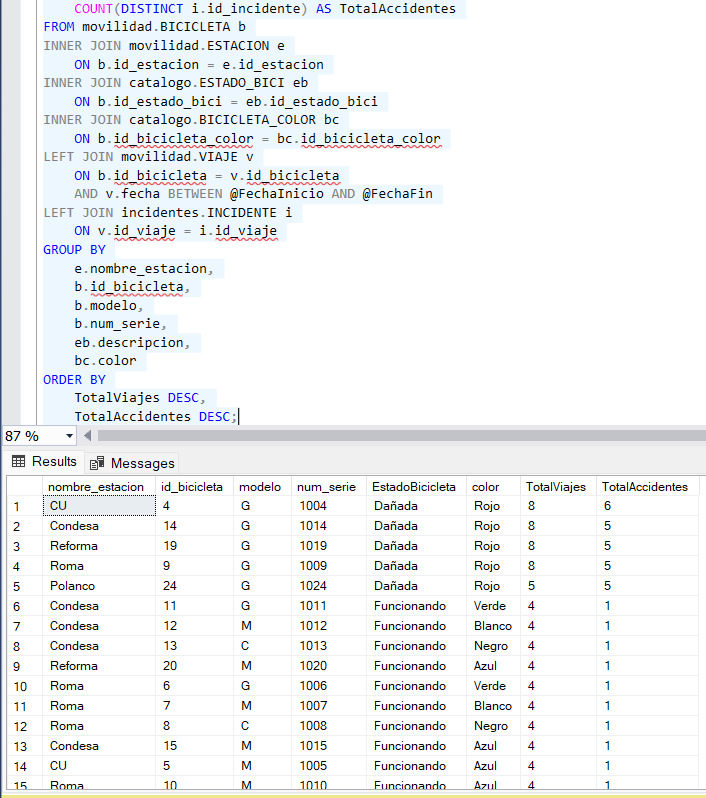
\includegraphics[width=0.85\textwidth]{figures/fig-009.png}
	\caption{Inventario de bicicletas por estación}
	\label{fig:est_6}
\end{figure}

\subsection{Estadística 7. Usuarios y antigüedad de membresía}

Esta consulta presenta la información general de los usuarios, el tipo de membresía que poseen y el tiempo que han permanecido suscritos al servicio en meses.

\begin{figure}[H]
	\centering
	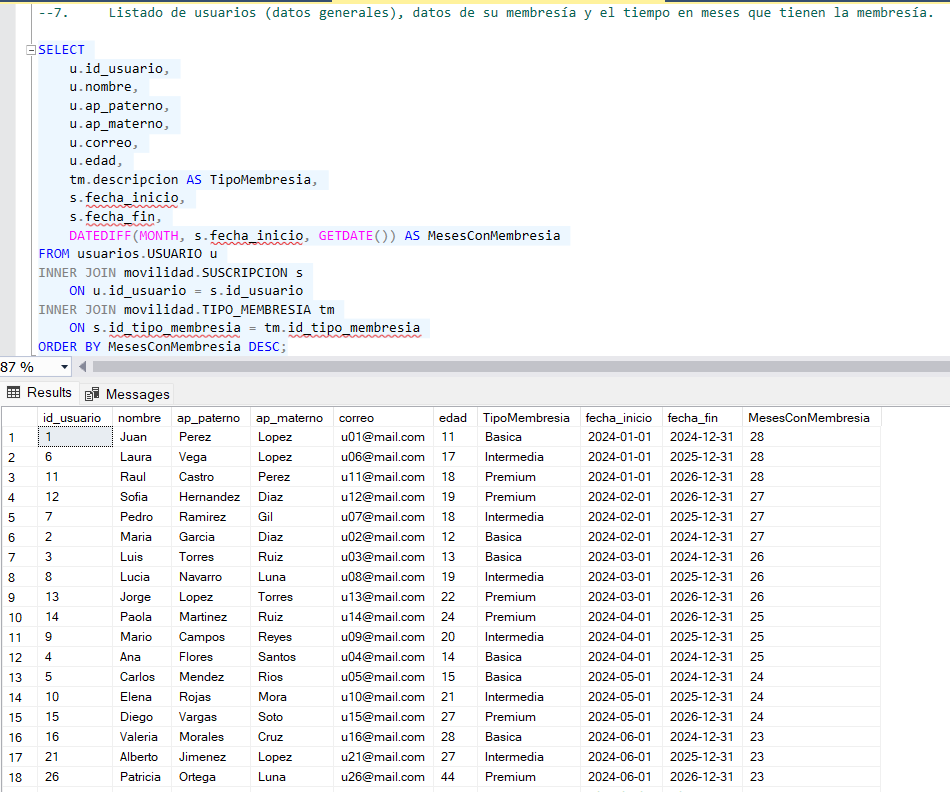
\includegraphics[width=0.85\textwidth]{figures/fig-010.png}
	\caption{Usuarios y antigüedad de membresía}
	\label{fig:est_7}
\end{figure}

\subsection{Estadística 8. Agentes mejor evaluados}

Esta consulta identifica a los agentes con mejor desempeño según las encuestas de satisfacción realizadas por los usuarios después de la atención de incidentes en un mes específico.

\begin{figure}[H]
	\centering
	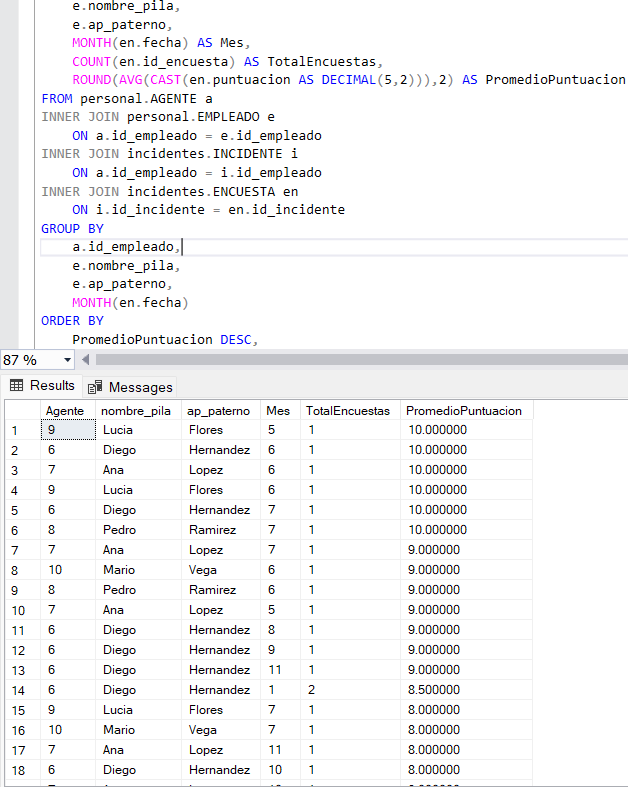
\includegraphics[width=0.85\textwidth]{figures/fig-011.png}
	\caption{Agentes mejor evaluados}
	\label{fig:est_8}
\end{figure}

\subsection{Estadística 9. Reporte diario de rondines}

Esta consulta genera un reporte diario de las actividades realizadas por el personal de rondín, incluyendo incidentes detectados, estación asociada y supervisor responsable (quien también es un empleado de rondines).

\begin{figure}[H]
	\centering
	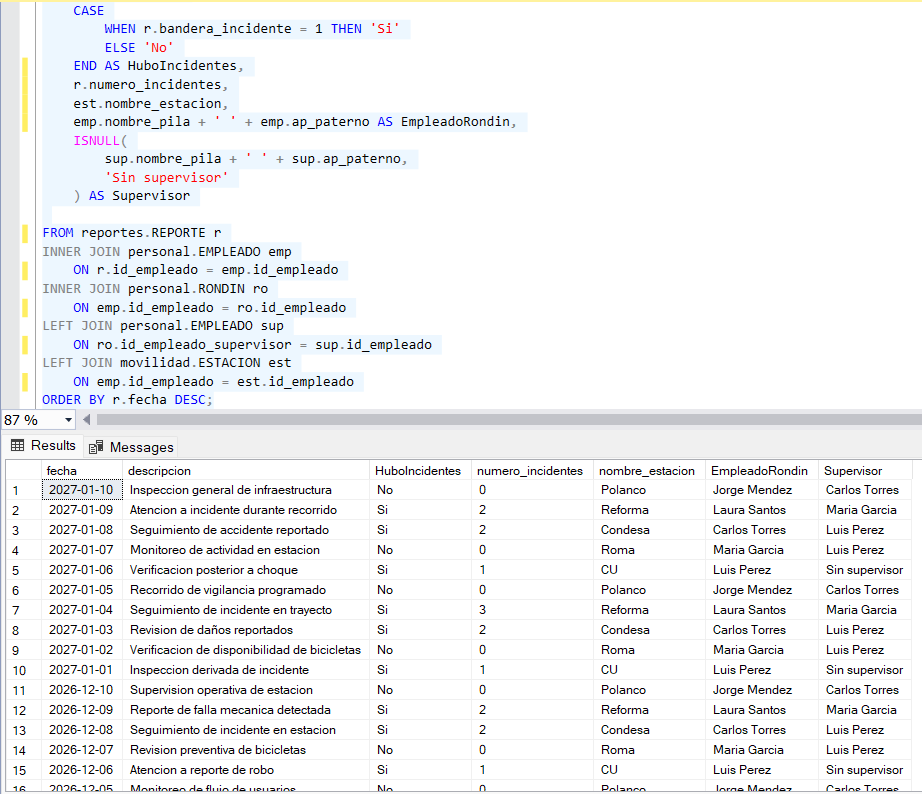
\includegraphics[width=0.85\textwidth]{figures/fig-012.png}
	\caption{Reporte diario de rondines}
	\label{fig:est_9}
\end{figure}

\subsection{Estadística 10. Listado completo de empleados}

Esta consulta muestra la información completa de los empleados registrados en el sistema, indicando además el tipo de puesto que desempeñan.

\begin{figure}[H]
	\centering
	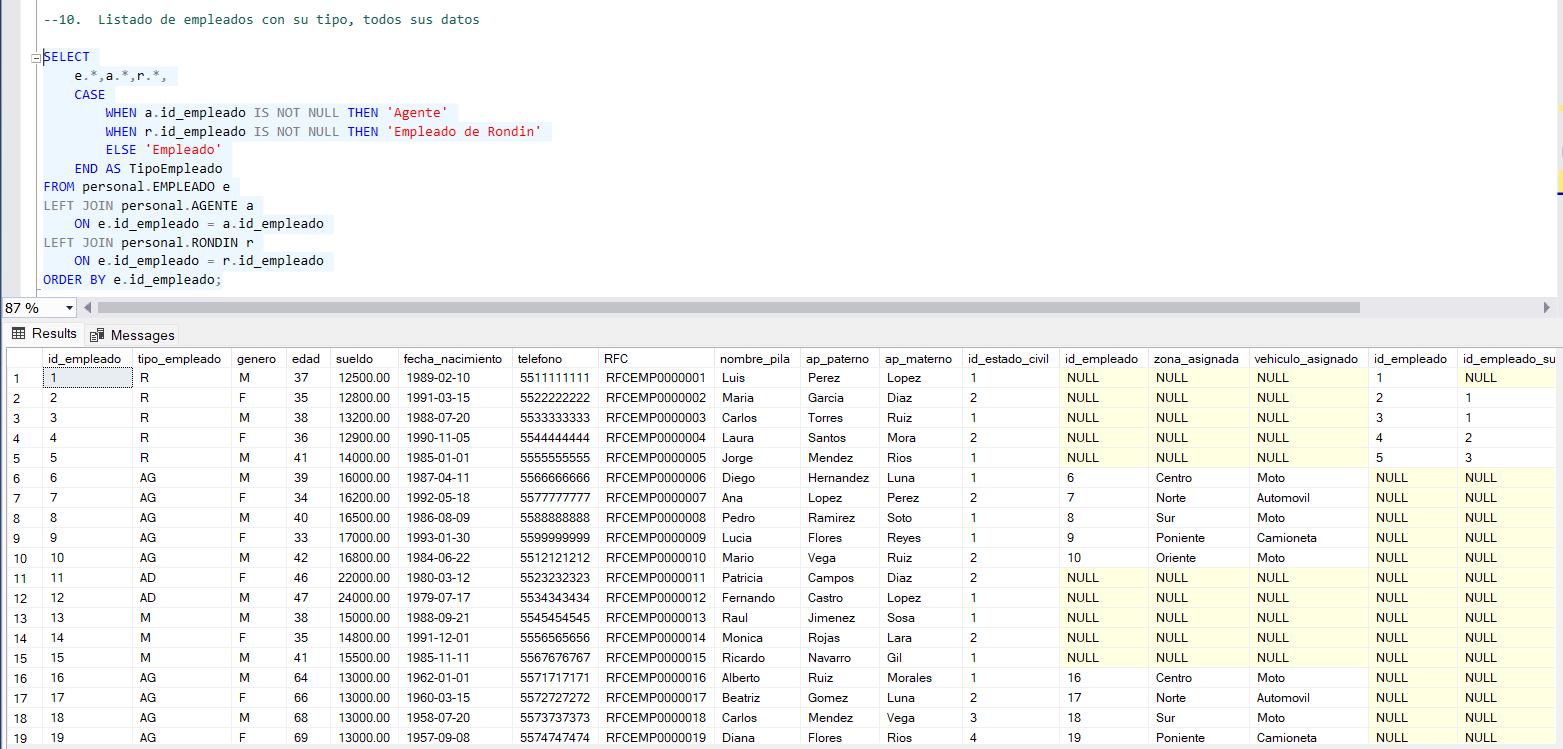
\includegraphics[width=0.85\textwidth]{figures/fig-013.png}
	\caption{Listado completo de empleados}
	\label{fig:est_10}
\end{figure}

\subsection{Estadística 11. Informe de recorridos}

Esta consulta genera un informe detallado de los viajes realizados por los usuarios, incluyendo estaciones de origen y destino, duración del recorrido y costo generado, en un periodo y/o estación determinada.

\begin{figure}[H]
	\centering
	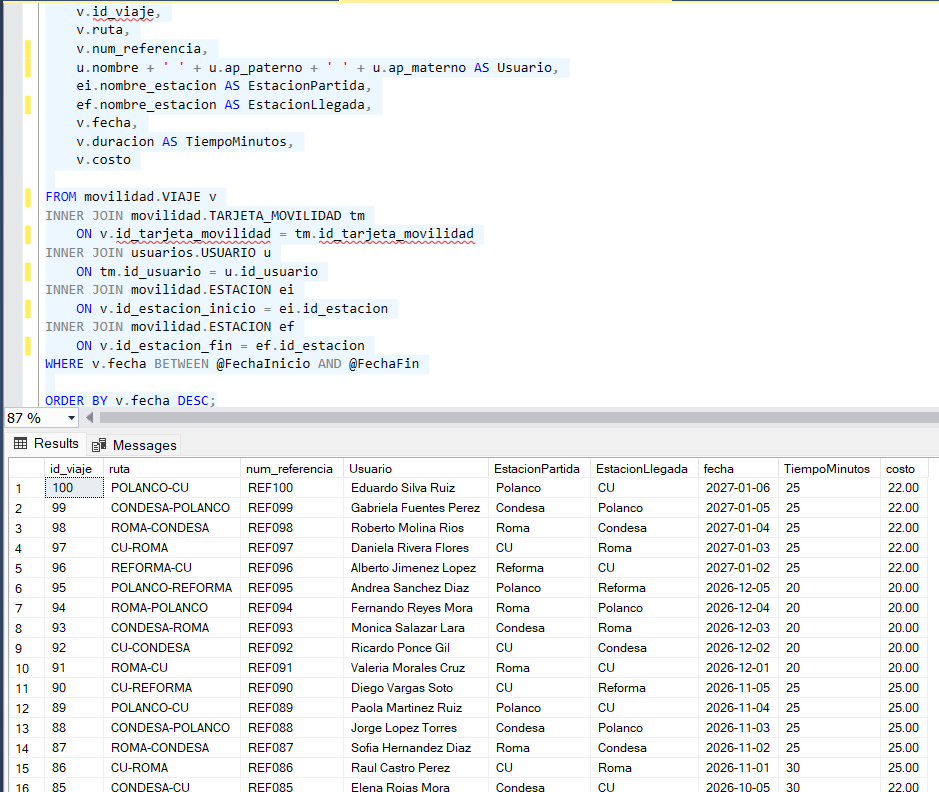
\includegraphics[width=0.85\textwidth]{figures/fig-014.png}
	\caption{Informe de recorridos}
	\label{fig:est_11}
\end{figure}

\subsection{Estadística 12. Recorridos por temporada}

Esta consulta permite conocer la cantidad de recorridos realizados durante cada temporada o época del año, identificando los periodos de mayor actividad ordenados de mayor a menor.

\begin{figure}[H]
	\centering
	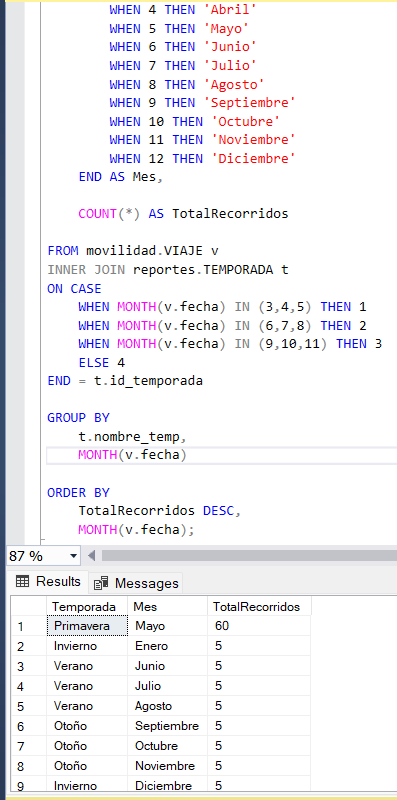
\includegraphics[width=0.85\textwidth]{figures/fig-015.png}
	\caption{Recorridos por temporada}
	\label{fig:est_12}
\end{figure}

\subsection{Estadística 13. Accidentes atendidos por agente}

Esta consulta muestra los datos personales de cada agente y el historial de accidentes que ha atendido, incluyendo fecha, lugar y tipo de incidente.

\begin{figure}[H]
	\centering
	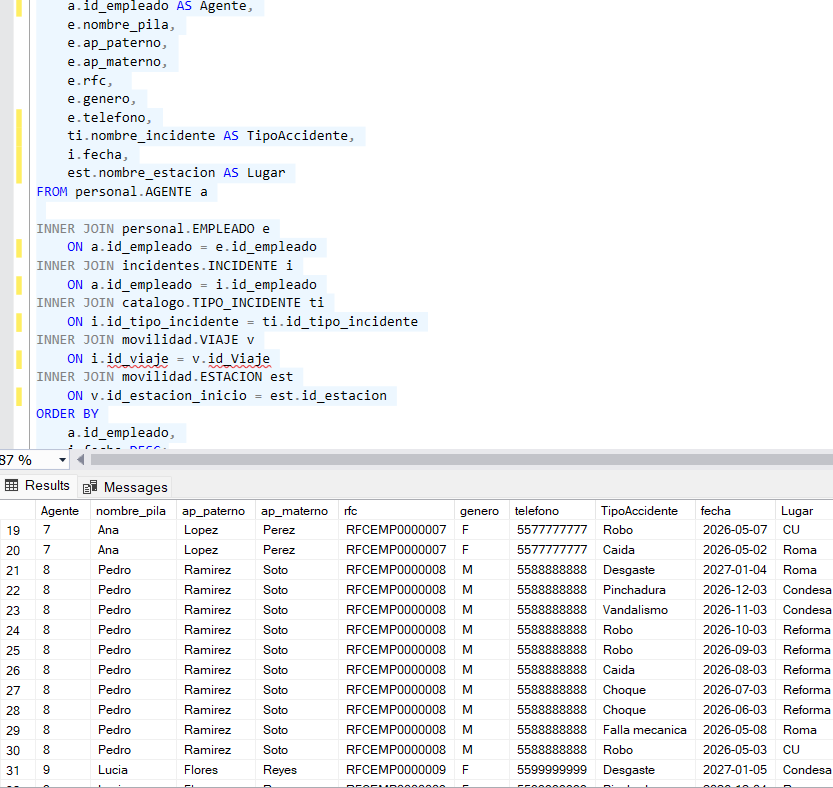
\includegraphics[width=0.85\textwidth]{figures/fig-016.png}
	\caption{Accidentes atendidos por agente}
	\label{fig:est_13}
\end{figure}

\subsection{Estadística 14. Informe de Recursos Humanos}

Esta consulta identifica empleados del área de administración que son de la tercera edad y que perciben un sueldo mensual de \$13,000, apoyando los procesos de análisis y gestión de recursos humanos.

\begin{figure}[H]
	\centering
	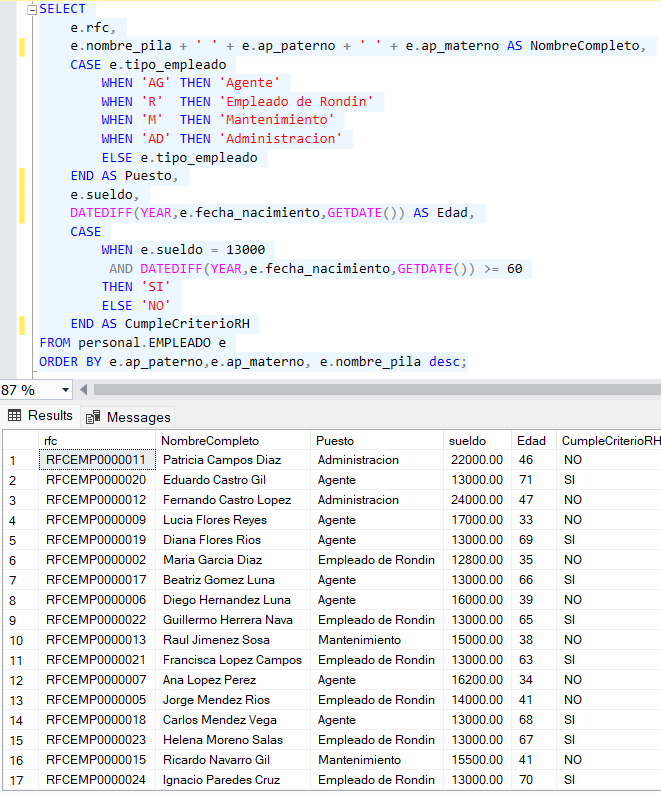
\includegraphics[width=0.85\textwidth]{figures/fig-017.png}
	\caption{Informe de Recursos Humanos}
	\label{fig:est_14}
\end{figure}

\subsection{Estadística 15. Faltas de empleados}

Esta consulta presenta estadísticas de faltas de empleados por periodo, clasificadas según el motivo registrado. La información permite analizar patrones de ausentismo dentro de la organización.

\begin{figure}[H]
	\centering
	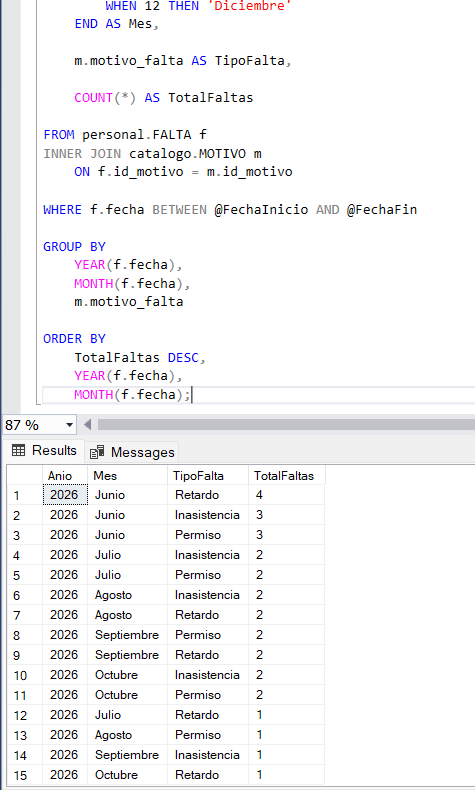
\includegraphics[width=0.85\textwidth]{figures/fig-018.png}
	\caption{Faltas de empleados}
	\label{fig:est_15}
\end{figure}

\section{Conclusiones}

\subsection{Conclusión General}

El desarrollo de la base de datos ECOBICI permitió aplicar de manera integral los conocimientos adquiridos durante el curso de Bases de Datos, abarcando las etapas de análisis, diseño conceptual, diseño lógico e implementación física. A lo largo del proyecto se construyó una solución capaz de administrar la información relacionada con usuarios, membresías, estaciones, bicicletas, viajes, incidentes y personal operativo, garantizando la integridad y consistencia de los datos mediante restricciones, llaves primarias, llaves foráneas y mecanismos de seguridad.

Asimismo, la implementación de procedimientos almacenados, funciones, vistas, triggers e informes estadísticos permitió automatizar procesos y facilitar la obtención de información relevante para la toma de decisiones. El proyecto permitió comprender la importancia de un diseño adecuado desde las primeras etapas de desarrollo, demostrando que una base de datos correctamente normalizada contribuye significativamente a la eficiencia, mantenimiento y escalabilidad de los sistemas de información.

\subsection{Conclusión de David Díaz Antúnez}

La realización de este proyecto permitió reforzar los conocimientos relacionados con el diseño e implementación de bases de datos relacionales, así como comprender la importancia de una correcta organización de la información para garantizar la integridad de los datos. Durante el desarrollo del sistema ECOBICI se adquirió experiencia en el uso de SQL Server, la creación de estructuras relacionales y la aplicación de buenas prácticas de modelado. Además, se fortalecieron habilidades de trabajo colaborativo y resolución de problemas, aspectos fundamentales en el desarrollo de proyectos de software.

\subsection{Conclusión de Mauricio Gabriel Hernández Acosta}

A través del desarrollo de la base de datos ECOBICI fue posible aplicar de manera práctica los conceptos estudiados durante el curso, especialmente aquellos relacionados con la normalización, la integridad referencial y la implementación de objetos programados. El proyecto permitió comprender cómo las decisiones tomadas durante la etapa de diseño impactan directamente en el rendimiento y mantenimiento de una base de datos. Asimismo, se obtuvo experiencia en la construcción de consultas complejas e informes estadísticos orientados al análisis de información y apoyo en la toma de decisiones.

\subsection{Conclusión de César Ricardo Sánchez Luján}

El proyecto ECOBICI representó una oportunidad para integrar conocimientos teóricos y prácticos en un entorno cercano a una situación real. La implementación de mecanismos de seguridad, restricciones de integridad y procesos automatizados permitió comprender la importancia de diseñar soluciones robustas y confiables. De igual forma, se fortaleció la capacidad para analizar requerimientos, modelar información y desarrollar bases de datos que satisfagan necesidades específicas de una organización, contribuyendo a la formación profesional en el área de tecnologías de la información.


\newpage
\section*{Bibliografía}
\addcontentsline{toc}{section}{Bibliografía}

\begin{thebibliography}{99}
	
	\bibitem{elmasri}
	R. Elmasri y S. B. Navathe, \textit{Fundamentals of Database Systems}. 7ma edición, Pearson, 2016.
	
	\bibitem{coronel}
	C. Coronel y S. Morris, \textit{Database Systems: Design, Implementation, \& Management}. 13va edición, Cengage Learning, 2019.
	
	\bibitem{silberschatz}
	A. Silberschatz, H. F. Korth y S. Sudarshan, \textit{Database System Concepts}. 7ma edición, McGraw-Hill Education, 2020.
	
	\bibitem{microsoft}
	Microsoft Corporation, \textit{SQL Server Documentation}. Recuperado de \url{https://learn.microsoft.com/sql}, 2025.
	
	\bibitem{date}
	C. J. Date, \textit{An Introduction to Database Systems}. 8va edición, Pearson, 2019.
	
	\bibitem{unam_fi}
	Universidad Nacional Autónoma de México, Facultad de Ingeniería, \textit{Material de apoyo y apuntes de la asignatura Bases de Datos}. Ciudad Universitaria, CDMX.
	
\end{thebibliography}
\newpage

\section{Anexos}
\label{sec:anexos}

Los siguientes documentos complementan la información presentada en esta documentación y contienen los elementos desarrollados durante la implementación del proyecto.

\subsection{Anexo A. Diccionario de Datos}
\label{sec:anexo_a}

El siguiente listado describe de manera detallada las tablas, campos, tipos de datos y descripciones asociadas que conforman la base de datos para la gestión del sistema ECOBICI.

\begingroup
\scriptsize
\renewcommand{\_}{\textunderscore\allowbreak}
\begin{longtable}{|p{3.2cm}|p{2.7cm}|p{3.0cm}|p{6.0cm}|}
	\hline
	\textbf{Tabla} & \textbf{Campo} & \textbf{Tipo de dato} & \textbf{Descripción} \\ \hline
	\endfirsthead
	\hline
	\textbf{Tabla} & \textbf{Campo} & \textbf{Tipo de dato} & \textbf{Descripción} \\ \hline
	\endhead
	\hline
	\endfoot
	\hline
	\endlastfoot
	
	% catalogo.ALCALDIA
	\texttt{catalogo.ALCALDIA} & \texttt{id\_alcaldia} & \texttt{INT} & Identificador único de alcaldía (Llave primaria). \\ \cline{2-4}
	& \texttt{alcaldia} & \texttt{VARCHAR(22)} & Nombre de la alcaldía. \\ \hline
	
	% catalogo.BICICLETA_COLOR
	\texttt{catalogo.BICICLETA\_COLOR} & \texttt{id\_bicicleta\_color} & \texttt{TINYINT} & Identificador único de color de bicicleta (Llave primaria). \\ \cline{2-4}
	& \texttt{color} & \texttt{VARCHAR(18)} & Descripción del color. \\ \hline
	
	% catalogo.ESTADO_BICI
	\texttt{catalogo.ESTADO\_BICI} & \texttt{id\_estado\_bici} & \texttt{INT} & Identificador único de estado de bicicleta (Llave primaria). \\ \cline{2-4}
	& \texttt{codigo} & \texttt{CHAR(1)} & Código representativo de estado (e.g. F, D, B). \\ \cline{2-4}
	& \texttt{descripcion} & \texttt{VARCHAR(20)} & Descripción larga del estado de la bicicleta. \\ \hline
	
	% catalogo.ESTADO_CIVIL
	\texttt{catalogo.ESTADO\_CIVIL} & \texttt{id\_estado\_civil} & \texttt{INT} & Identificador único de estado civil (Llave primaria). \\ \cline{2-4}
	& \texttt{codigo} & \texttt{CHAR(1)} & Código corto del estado civil (e.g. S, C, O). \\ \cline{2-4}
	& \texttt{estado\_civil} & \texttt{VARCHAR(15)} & Nombre descriptivo del estado civil (e.g. Concubinato). \\ \cline{2-4}
	& \texttt{vigente} & \texttt{BIT} & Indica si el estado civil sigue activo o vigente en el catálogo. \\ \hline
	
	% catalogo.CATALOGO_IDIOMAS
	\texttt{catalogo.CATALOGO\_IDIOMAS} & \texttt{id\_idioma} & \texttt{INT} & Identificador único de idioma (Llave primaria). \\ \cline{2-4}
	& \texttt{nombre\_idioma} & \texttt{VARCHAR(30)} & Nombre del idioma (e.g. Inglés, Francés). \\ \hline
	
	% catalogo.ESPECIALIDAD
	\texttt{catalogo.ESPECIALIDAD} & \texttt{id\_especialidad} & \texttt{INT} & Identificador único de especialidad (Llave primaria). \\ \cline{2-4}
	& \texttt{especialidad} & \texttt{VARCHAR(25)} & Nombre de la especialidad del mecánico. \\ \hline
	
	% catalogo.MOTIVO
	\texttt{catalogo.MOTIVO} & \texttt{id\_motivo} & \texttt{INT} & Identificador único del motivo (Llave primaria). \\ \cline{2-4}
	& \texttt{motivo\_falta} & \texttt{VARCHAR(30)} & Causa de falta justificada o no para empleados. \\ \hline
	
	% catalogo.TIPO_INCIDENTE
	\texttt{catalogo.TIPO\_INCIDENTE} & \texttt{id\_tipo\_incidente} & \texttt{INT} & Identificador único del tipo de incidente (Llave primaria). \\ \cline{2-4}
	& \texttt{nombre\_incidente} & \texttt{VARCHAR(30)} & Nombre corto del tipo de incidente vial o mecánico. \\ \cline{2-4}
	& \texttt{descripcion} & \texttt{VARCHAR(80)} & Descripción del incidente. \\ \hline
	
	% personal.EMPLEADO
	\texttt{personal.EMPLEADO} & \texttt{id\_empleado} & \texttt{INT} & Identificador único de empleado (Llave primaria). \\ \cline{2-4}
	& \texttt{tipo\_empleado} & \texttt{VARCHAR(2)} & Código de tipo (A = Agente, R = Rondines, D = Administrador, M = Mantenimiento). \\ \cline{2-4}
	& \texttt{genero} & \texttt{CHAR(1)} & Género del empleado (M, F). \\ \cline{2-4}
	& \texttt{edad} & \texttt{INT (Calculado)} & Edad del empleado calculada a partir de su fecha de nacimiento. \\ \cline{2-4}
	& \texttt{sueldo} & \texttt{DECIMAL(12,2)} & Sueldo mensual bruto del empleado. \\ \cline{2-4}
	& \texttt{fecha\_nacimiento} & \texttt{DATE} & Fecha de nacimiento del empleado. \\ \cline{2-4}
	& \texttt{telefono} & \texttt{NUMERIC(10,0)} & Número telefónico personal de contacto. \\ \cline{2-4}
	& \texttt{RFC} & \texttt{CHAR(13)} & Registro Federal de Contribuyentes único. \\ \cline{2-4}
	& \texttt{nombre\_pila} & \texttt{VARCHAR(30)} & Nombre o nombres de pila. \\ \cline{2-4}
	& \texttt{ap\_paterno} & \texttt{VARCHAR(30)} & Apellido paterno. \\ \cline{2-4}
	& \texttt{ap\_materno} & \texttt{VARCHAR(30)} & Apellido materno. \\ \cline{2-4}
	& \texttt{id\_estado\_civil} & \texttt{INT} & Relación con catálogo de estados civiles (Llave foránea). \\ \hline
	
	% personal.ADMINISTRACION
	\texttt{personal.ADMINISTRACION} & \texttt{id\_empleado} & \texttt{INT} & Identificador del empleado administrativo (Llave primaria / foránea). \\ \cline{2-4}
	& \texttt{profesion} & \texttt{VARCHAR(30)} & Profesión o carrera universitaria del empleado. \\ \cline{2-4}
	& \texttt{ubicacion\_trabajo} & \texttt{VARCHAR(40)} & Nombre del área u oficina física asignada. \\ \hline
	
	% personal.AGENTE
	\texttt{personal.AGENTE} & \texttt{id\_empleado} & \texttt{INT} & Identificador del agente de incidentes (Llave primaria / foránea). \\ \cline{2-4}
	& \texttt{zona\_asignada} & \texttt{VARCHAR(30)} & Zona vial asignada para su cobertura. \\ \cline{2-4}
	& \texttt{vehiculo\_asignado} & \texttt{VARCHAR(20)} & Placa o código del vehículo de patrullaje asignado. \\ \hline
	
	% personal.RONDIN
	\texttt{personal.RONDIN} & \texttt{id\_empleado} & \texttt{INT} & Identificador del personal de rondín (Llave primaria / foránea). \\ \cline{2-4}
	& \texttt{id\_empleado\_supervisor} & \texttt{INT} & Identificador del supervisor de rondín (Llave foránea a la misma tabla). \\ \hline
	
	% personal.MANTENIMIENTO
	\texttt{personal.MANTENIMIENTO} & \texttt{id\_empleado} & \texttt{INT} & Identificador del mecánico de mantenimiento (Llave primaria / foránea). \\ \cline{2-4}
	& \texttt{id\_especialidad} & \texttt{INT} & Relación con especialidad (Llave foránea). \\ \hline
	
	% personal.COLONIA
	\texttt{personal.COLONIA} & \texttt{id\_colonia} & \texttt{INT} & Identificador único de la colonia (Llave primaria). \\ \cline{2-4}
	& \texttt{colonia} & \texttt{VARCHAR(20)} & Nombre oficial de la colonia. \\ \cline{2-4}
	& \texttt{id\_alcaldia} & \texttt{INT} & Relación con alcaldía (Llave foránea). \\ \hline
	
	% personal.DOMICILIO
	\texttt{personal.DOMICILIO} & \texttt{id\_empleado} & \texttt{INT} & Identificador del empleado (Llave primaria / foránea). \\ \cline{2-4}
	& \texttt{id\_domicilio} & \texttt{INT} & Identificador único de domicilio (Llave primaria). \\ \cline{2-4}
	& \texttt{numero\_ext} & \texttt{NUMERIC(3,0)} & Número exterior del domicilio. \\ \cline{2-4}
	& \texttt{numero\_int} & \texttt{NUMERIC(3,0)} & Número interior (opcional). \\ \cline{2-4}
	& \texttt{calle} & \texttt{VARCHAR(30)} & Calle de residencia. \\ \cline{2-4}
	& \texttt{id\_colonia} & \texttt{INT} & Relación con colonia (Llave foránea). \\ \hline
	
	% personal.IDIOMAS
	\texttt{personal.IDIOMAS} & \texttt{id\_empleado} & \texttt{INT} & Identificador del empleado (Llave primaria / foránea). \\ \cline{2-4}
	& \texttt{id\_idioma} & \texttt{INT} & Relación con el catálogo de idiomas (Llave primaria / foránea). \\ \hline
	
	% personal.FALTA
	\texttt{personal.FALTA} & \texttt{id\_empleado} & \texttt{INT} & Identificador del empleado faltante (Llave primaria / foránea). \\ \cline{2-4}
	& \texttt{id\_falta} & \texttt{SMALLINT} & Consecutivo de falta individual por empleado (Llave primaria). \\ \cline{2-4}
	& \texttt{fecha} & \texttt{DATE} & Fecha del ausentismo. \\ \cline{2-4}
	& \texttt{id\_motivo} & \texttt{INT} & Relación con motivo de falta (Llave foránea). \\ \hline
	
	% personal.FUNCIONES
	\texttt{personal.FUNCIONES} & \texttt{id\_funciones} & \texttt{INT} & Identificador único de la función del empleado (Llave primaria). \\ \cline{2-4}
	& \texttt{id\_empleado} & \texttt{INT} & Relación con el empleado asignado (Llave foránea). \\ \cline{2-4}
	& \texttt{nombre\_funcion} & \texttt{VARCHAR(30)} & Nombre descriptivo del puesto o función. \\ \hline
	
	% usuarios.USUARIO
	\texttt{usuarios.USUARIO} & \texttt{id\_usuario} & \texttt{INT} & Identificador único de usuario del sistema (Llave primaria). \\ \cline{2-4}
	& \texttt{correo} & \texttt{VARCHAR(30)} & Correo electrónico único del usuario. \\ \cline{2-4}
	& \texttt{nombre} & \texttt{VARCHAR(40)} & Nombre o nombres de pila. \\ \cline{2-4}
	& \texttt{ap\_paterno} & \texttt{VARCHAR(40)} & Apellido paterno. \\ \cline{2-4}
	& \texttt{ap\_materno} & \texttt{VARCHAR(40)} & Apellido materno. \\ \cline{2-4}
	& \texttt{codigo\_INE} & \texttt{CHAR(18)} & Código INE oficial de identificación del usuario. \\ \cline{2-4}
	& \texttt{fecha\_nacimiento} & \texttt{DATE} & Fecha de nacimiento del usuario. \\ \cline{2-4}
	& \texttt{genero} & \texttt{CHAR(1)} & Género del usuario (M o F). \\ \cline{2-4}
	& \texttt{edad} & \texttt{INT (Calculado)} & Edad del usuario calculada a partir de su fecha de nacimiento. \\ \hline
	
	% usuarios.TELEFONO
	\texttt{usuarios.TELEFONO} & \texttt{id\_telefono} & \texttt{INT} & Identificador único de teléfono (Llave primaria). \\ \cline{2-4}
	& \texttt{id\_usuario} & \texttt{INT} & Relación con usuario (Llave foránea). \\ \cline{2-4}
	& \texttt{telefono} & \texttt{CHAR(10)} & Número de teléfono de contacto (10 dígitos). \\ \hline
	
	% movilidad.METODO_PAGO
	\texttt{movilidad.METODO\_PAGO} & \texttt{id\_metodo\_pago} & \texttt{INT} & Identificador único del método de pago (Llave primaria). \\ \cline{2-4}
	& \texttt{fecha\_exp} & \texttt{DATE} & Fecha de expiración del medio de pago electrónico (e.g. Tarjeta). \\ \cline{2-4}
	& \texttt{fecha\_inicio} & \texttt{DATE} & Fecha de registro inicial. \\ \cline{2-4}
	& \texttt{tipo\_pago} & \texttt{CHAR(1)} & Clave representativa del tipo de pago (e.g. C = Crédito, D = Débito). \\ \hline
	
	% movilidad.TIPO_MEMBRESIA
	\texttt{movilidad.TIPO\_MEMBRESIA} & \texttt{id\_tipo\_membresia} & \texttt{INT} & Identificador de tipo de membresía (Llave primaria). \\ \cline{2-4}
	& \texttt{tipo\_membresia} & \texttt{CHAR(1)} & Código corto del tipo de membresía (B = Básica, I = Intermedia, P = Premium). \\ \cline{2-4}
	& \texttt{descripcion} & \texttt{VARCHAR(15)} & Nombre descriptivo del plan de membresía. \\ \cline{2-4}
	& \texttt{duracion\_dias} & \texttt{NUMERIC(4,0)} & Cantidad de días de vigencia de la suscripción. \\ \cline{2-4}
	& \texttt{tipo\_seguro} & \texttt{CHAR(1)} & Categoría del seguro médico/vial incluido. \\ \cline{2-4}
	& \texttt{tiempo\_excedente} & \texttt{DECIMAL(18,0)} & Tiempo libre de viaje permitido en minutos. \\ \cline{2-4}
	& \texttt{costo\_base} & \texttt{DECIMAL(10,2)} & Costo fijo de contratación del plan. \\ \cline{2-4}
	& \texttt{tarifa\_excedente} & \texttt{DECIMAL(10,2)} & Costo cobrado por cada minuto excedido. \\ \cline{2-4}
	& \texttt{tipo\_beneficio} & \texttt{CHAR(1)} & Código interno de beneficios adicionales. \\ \hline
	
	% movilidad.SUSCRIPCION
	\texttt{movilidad.SUSCRIPCION} & \texttt{id\_suscripcion} & \texttt{INT} & Identificador único de suscripción (Llave primaria). \\ \cline{2-4}
	& \texttt{estado} & \texttt{CHAR(1)} & Estado de la suscripción (e.g. A = Activa, C = Cancelada). \\ \cline{2-4}
	& \texttt{fecha\_fin} & \texttt{DATE} & Fecha en la que vence o finaliza la suscripción. \\ \cline{2-4}
	& \texttt{fecha\_inicio} & \texttt{DATE} & Fecha de alta o renovación de la suscripción. \\ \cline{2-4}
	& \texttt{id\_usuario} & \texttt{INT} & Relación con el usuario contratante (Llave foránea). \\ \cline{2-4}
	& \texttt{id\_metodo\_pago} & \texttt{INT} & Relación con el medio de pago activo (Llave foránea). \\ \cline{2-4}
	& \texttt{id\_tipo\_membresia} & \texttt{INT} & Relación con el tipo de membresía contratado (Llave foránea). \\ \hline
	
	% movilidad.TARJETA_MOVILIDAD
	\texttt{movilidad.TARJETA\_MOVILIDAD} & \texttt{id\_tarjeta\_movilidad} & \texttt{INT} & Identificador físico único de la tarjeta de movilidad integrada (Llave primaria). \\ \cline{2-4}
	& \texttt{id\_tarjeta\_reposicion} & \texttt{INT} & Enlace a la tarjeta anterior que fue reemplazada (Llave foránea a la misma tabla). \\ \cline{2-4}
	& \texttt{id\_usuario} & \texttt{INT} & Relación con el usuario propietario (Llave foránea). \\ \cline{2-4}
	& \texttt{fecha\_baja} & \texttt{DATE} & Fecha en la que se desactivó la tarjeta. \\ \cline{2-4}
	& \texttt{saldo} & \texttt{DECIMAL(10,2)} & Saldo cargado disponible en la tarjeta. \\ \cline{2-4}
	& \texttt{codigo\_QR} & \texttt{VARBINARY(100)} & Código binario del QR impreso en la tarjeta. \\ \cline{2-4}
	& \texttt{fecha\_emision} & \texttt{DATE} & Fecha de expedición de la tarjeta. \\ \cline{2-4}
	& \texttt{activa} & \texttt{BIT} & Indica si la tarjeta está operativa (1) o inactiva (0). \\ \cline{2-4}
	& \texttt{tipo\_emision} & \texttt{VARCHAR(20)} & Tipo de expedición de la tarjeta (e.g. Primera vez, Reposición). \\ \hline
	
	% movilidad.ESTACION
	\texttt{movilidad.ESTACION} & \texttt{id\_estacion} & \texttt{INT} & Identificador único de estación de servicio (Llave primaria). \\ \cline{2-4}
	& \texttt{terminales\_disponibles} & \texttt{INT} & Puertos o anclajes libres para recibir bicicletas. \\ \cline{2-4}
	& \texttt{terminales\_totales} & \texttt{INT} & Capacidad máxima de anclajes en la estación. \\ \cline{2-4}
	& \texttt{nombre\_estacion} & \texttt{VARCHAR(20)} & Nombre público de la estación. \\ \cline{2-4}
	& \texttt{id\_empleado} & \texttt{INT} & Mecánico de mantenimiento responsable asignado (Llave foránea). \\ \hline
	
	% movilidad.BICICLETA
	\texttt{movilidad.BICICLETA} & \texttt{id\_bicicleta} & \texttt{INT} & Identificador único de bicicleta (Llave primaria). \\ \cline{2-4}
	& \texttt{modelo} & \texttt{CHAR(1)} & Categoría de tamaño de la unidad (C = Chica, M = Mediana, G = Grande). \\ \cline{2-4}
	& \texttt{num\_serie} & \texttt{NUMERIC(10,0)} & Número de serie grabado único de la bicicleta. \\ \cline{2-4}
	& \texttt{id\_estado\_bici} & \texttt{INT} & Relación con catálogo de estados de bicicleta (Llave foránea). \\ \cline{2-4}
	& \texttt{id\_estacion} & \texttt{INT} & Estación física actual donde se ancla la bicicleta (Llave foránea). \\ \cline{2-4}
	& \texttt{id\_bicicleta\_color} & \texttt{TINYINT} & Relación con catálogo de colores de bicicleta (Llave foránea). \\ \hline
	
	% movilidad.VIAJE
	\texttt{movilidad.VIAJE} & \texttt{id\_viaje} & \texttt{INT} & Identificador único del viaje (Llave primaria). \\ \cline{2-4}
	& \texttt{costo} & \texttt{DECIMAL(10,2)} & Cargo final cobrado al usuario (base + excedente). \\ \cline{2-4}
	& \texttt{fecha} & \texttt{DATE} & Fecha del recorrido. \\ \cline{2-4}
	& \texttt{ruta} & \texttt{VARCHAR(60)} & Descripción de la trayectoria aproximada. \\ \cline{2-4}
	& \texttt{hora\_inicio} & \texttt{DATETIME} & Hora en la que se liberó la bicicleta del anclaje. \\ \cline{2-4}
	& \texttt{hora\_fin} & \texttt{DATETIME} & Hora en la que se aseguró la bicicleta en la estación de destino. \\ \cline{2-4}
	& \texttt{duracion} & \texttt{INT (Calculado)} & Duración en minutos calculada a partir de las horas de inicio y fin. \\ \cline{2-4}
	& \texttt{num\_referencia} & \texttt{VARCHAR(20)} & Folio o código de transacción bancaria / operativa. \\ \cline{2-4}
	& \texttt{id\_bicicleta} & \texttt{INT} & Relación con la bicicleta prestada (Llave foránea). \\ \cline{2-4}
	& \texttt{id\_estacion\_inicio} & \texttt{INT} & Estación origen (Llave foránea). \\ \cline{2-4}
	& \texttt{id\_estacion\_fin} & \texttt{INT} & Estación destino (Llave foránea). \\ \cline{2-4}
	& \texttt{id\_tarjeta\_movilidad} & \texttt{INT} & Tarjeta de movilidad con la que se inició el viaje (Llave foránea). \\ \hline
	
	% incidentes.INCIDENTE
	\texttt{incidentes.INCIDENTE} & \texttt{id\_incidente} & \texttt{INT} & Identificador de reporte de incidente (Llave primaria). \\ \cline{2-4}
	& \texttt{calle} & \texttt{VARCHAR(30)} & Vialidad donde ocurrió el incidente. \\ \cline{2-4}
	& \texttt{numero} & \texttt{NUMERIC(4,0)} & Altura o número aproximado del lugar del incidente. \\ \cline{2-4}
	& \texttt{codigo\_postal} & \texttt{NUMERIC(5,0)} & Código postal de la zona. \\ \cline{2-4}
	& \texttt{fecha} & \texttt{DATE} & Fecha del reporte. \\ \cline{2-4}
	& \texttt{latitud} & \texttt{VARCHAR(20)} & Coordenada de latitud geográfica. \\ \cline{2-4}
	& \texttt{longitud} & \texttt{VARCHAR(20)} & Coordenada de longitud geográfica. \\ \cline{2-4}
	& \texttt{id\_viaje} & \texttt{INT} & Relación con el viaje en el que se reportó el percance (Llave foránea). \\ \cline{2-4}
	& \texttt{id\_tipo\_incidente} & \texttt{INT} & Relación con tipo de incidente (Llave foránea). \\ \cline{2-4}
	& \texttt{id\_empleado} & \texttt{INT} & Agente de incidentes responsable de la atención (Llave foránea). \\ \cline{2-4}
	& \texttt{id\_colonia} & \texttt{INT} & Relación con la colonia asociada (Llave foránea). \\ \hline
	
	% incidentes.ENCUESTA
	\texttt{incidentes.ENCUESTA} & \texttt{id\_encuesta} & \texttt{INT} & Identificador de encuesta (Llave primaria). \\ \cline{2-4}
	& \texttt{id\_incidente} & \texttt{INT} & Relación con el incidente calificado (Llave foránea). \\ \cline{2-4}
	& \texttt{puntuacion} & \texttt{NUMERIC(2,0)} & Calificación asignada al agente (rango de 1 a 10). \\ \cline{2-4}
	& \texttt{fecha} & \texttt{DATE} & Fecha de la encuesta. \\ \cline{2-4}
	& \texttt{comentario} & \texttt{VARCHAR(120)} & Comentarios adicionales del usuario. \\ \hline
	
	% reportes.TEMPORADA
	\texttt{reportes.TEMPORADA} & \texttt{id\_temporada} & \texttt{INT} & Identificador único de temporada del año (Llave primaria). \\ \cline{2-4}
	& \texttt{nombre\_temp} & \texttt{VARCHAR(15)} & Nombre de la estación (e.g. Primavera, Invierno, Lluvias). \\ \hline
	
	% reportes.REPORTE
	\texttt{reportes.REPORTE} & \texttt{id\_reporte} & \texttt{INT} & Identificador único de reporte operativo (Llave primaria). \\ \cline{2-4}
	& \texttt{fecha} & \texttt{DATE} & Fecha en la que se generó el reporte. \\ \cline{2-4}
	& \texttt{descripcion} & \texttt{VARCHAR(90)} & Descripción de las observaciones realizadas. \\ \cline{2-4}
	& \texttt{bandera\_incidente} & \texttt{BIT} & Indica si se detectaron incidentes graves viales (1) o no (0). \\ \cline{2-4}
	& \texttt{numero\_incidentes} & \texttt{NUMERIC(2,0)} & Número total de incidentes reportados en el día. \\ \cline{2-4}
	& \texttt{id\_empleado} & \texttt{INT} & Empleado de rondines que genera el reporte (Llave foránea). \\ \cline{2-4}
	& \texttt{id\_temporada} & \texttt{INT} & Relación con la temporada climática actual (Llave foránea). \\ \hline
\end{longtable}
\endgroup

\newpage

\subsection{Anexo B. Script de Seguridad}
\label{sec:anexo_b}
En este anexo se presenta la implementación de la capa de seguridad a nivel de base de datos, la cual define roles, usuarios y permisos.

\inputencoding{cp1252}
\lstinputlisting[style=sqlstyle]{../scripts/seguridad.sql}
\inputencoding{utf8}

\newpage

\subsection{Anexo C. Script de Creación de la Base de Datos}
\label{sec:anexo_c}
En este anexo se incluye el script DDL encargado de crear la estructura lógica del sistema ECOBICI.

\inputencoding{cp1252}
\lstinputlisting[style=sqlstyle]{../scripts/creaBase.sql}
\inputencoding{utf8}

\newpage

\subsection{Anexo D. Script de Objetos Programados}
\label{sec:anexo_d}
En este anexo se presenta la lógica programada (procedimientos almacenados, funciones, disparadores y vistas) del sistema.

\inputencoding{cp1252}
\lstinputlisting[style=sqlstyle]{../scripts/dml.sql}
\inputencoding{utf8}

\newpage

\subsection{Anexo E. Script de Carga Inicial}
\label{sec:anexo_e}
En este anexo se incluye la carga de datos maestros e históricos iniciales que permiten el testeo del sistema.

\inputencoding{cp1252}
\lstinputlisting[style=sqlstyle]{../scripts/cargaInicial.sql}
\inputencoding{utf8}

\newpage

\subsection{Anexo F. Script de Informes y Estadísticas}
\label{sec:anexo_f}
En este anexo se detallan las quince consultas analíticas ejecutadas sobre la base de datos de ECOBICI.

\inputencoding{cp1252}
\lstinputlisting[style=sqlstyle]{../scripts/informes.sql}
\inputencoding{utf8}


\end{document}
